%%%%%%%%%%%%%%%%%%%%%%%%%%%%%%%%%%%%%%%%%%%%%%%%%%%%%%%%%%%%%%%%%%%%% 
%% This is a (brief) model paper using the achemso class 
%% The document class accepts keyval options, which should include 
%% the target journal and optionally the manuscript type. 
%%%%%%%%%%%%%%%%%%%%%%%%%%%%%%%%%%%%%%%%%%%%%%%%%%%%%%%%%%%%%%%%%%%%% 
\documentclass[journal=jpcbfk,manuscript=article]{achemso} 
 
%%%%%%%%%%%%%%%%%%%%%%%%%%%%%%%%%%%%%%%%%%%%%%%%%%%%%%%%%%%%%%%%%%%%% 
%% Place any additional packages needed here.  Only include packages 
%% which are essential, to avoid problems later. Do NOT use any 
%% packages which require e-TeX (for example etoolbox): the e-TeX 
%% extensions are not currently available on the ACS conversion 
%% servers. 
%%%%%%%%%%%%%%%%%%%%%%%%%%%%%%%%%%%%%%%%%%%%%%%%%%%%%%%%%%%%%%%%%%%%% 

%% Workaround for malfunctioning textsuperscript with pdfx and T1 encoding
\let\tmpa\textsuperscript
\DeclareTextCommandDefault{\textsuperscript}{\tmpa}

\usepackage[x11names]{xcolor}  % typesetting in color
%% Generate PDF/A-2u
\usepackage[a-2u]{pdfx}
 
\usepackage[super]{natbib}         % citation style AUTHOR (YEAR), or AUTHOR [NUMBER]

\usepackage{achemso}  
\usepackage{rotating}  
%\usepackage{times} 
%\usepackage{lmodern}    %% Prefer Latin Modern fonts
\usepackage{graphicx} 
\usepackage{setspace} 
\usepackage{amsmath} 
\usepackage{epstopdf} 
\usepackage{csquotes} 
\usepackage{mhchem} 
\usepackage{chemfig} 
\usepackage[obeyFinal]{easy-todo}
\usepackage[english]{babel}
 
\usepackage{subfig}
\usepackage{dcolumn}        % improved alignment of table columns
\usepackage{booktabs}       % improved horizontal lines in tables
\usepackage{paralist}       % improved enumerate and itemize

%% Character encoding: usually latin2, cp1250 or utf8:
\usepackage[utf8]{inputenc}
\usepackage[T1]{fontenc}

%\usepackage{markdown}  
 
%% The hyperref package for clickable links in PDF and also for storing
%% metadata to PDF (including the table of contents).
%% Most settings are pre-set by the pdfx package.
\hypersetup{unicode}
\hypersetup{breaklinks=true}
\hypersetup{colorlinks,allcolors=DodgerBlue4}
 
%%%%%%%%%%%%%%%%%%%%%%%%%%%%%%%%%%%%%%%%%%%%%%%%%%%%%%%%%%%%%%%%%%%%% 
%% If issues arise when submitting your manuscript, you may want to 
%% un-comment the next line.  This provides information on the 
%% version of every file you have used. 
%%%%%%%%%%%%%%%%%%%%%%%%%%%%%%%%%%%%%%%%%%%%%%%%%%%%%%%%%%%%%%%%%%%%% 
%%\listfiles 
 
%%%%%%%%%%%%%%%%%%%%%%%%%%%%%%%%%%%%%%%%%%%%%%%%%%%%%%%%%%%%%%%%%%%%% 
%% Place any additional macros here.  Please use \newcommand* where 
%% possible, and avoid layout-changing macros (which are not used 
%% when typesetting). 
%%%%%%%%%%%%%%%%%%%%%%%%%%%%%%%%%%%%%%%%%%%%%%%%%%%%%%%%%%%%%%%%%%%%% 
\newcommand*\mycommand[1]{\texttt{\emph{#1}}} 
%%% Custom variables
% width suitable for fitting into a column in 1-column page layout
\newlength{\figwidth}
\setlength{\figwidth}{9 cm} 
\newlength{\figwidthsmall}
\setlength{\figwidthsmall}{6 cm} 
\newlength{\figwidthfull}
\setlength{\figwidthfull}{14 cm} 

 
%%%%%%%%%%%%%%%%%%%%%%%%%%%%%%%%%%%%%%%%%%%%%%%%%%%%%%%%%%%%%%%%%%%%% 
%% Meta-data block 
%% --------------- 
%% Each author should be given as a separate \author command. 
%% 
%% Corresponding authors should have an e-mail given after the author 
%% name as an \email command. Phone and fax numbers can be given 
%% using \phone and \fax, respectively; this information is optional. 
%% 
%% The affiliation of authors is given after the authors; each 
%% \affiliation command applies to all preceding authors not already 
%% assigned an affiliation. 
%% 
%% The affiliation takes an option argument for the short name.  This 
%% will typically be something like "University of Somewhere". 
%% 
%% The \altaffiliation macro should be used for new address, etc. 
%% On the other hand, \alsoaffiliation is used on a per author basis 
%% when authors are associated with multiple institutions. 
%%%%%%%%%%%%%%%%%%%%%%%%%%%%%%%%%%%%%%%%%%%%%%%%%%%%%%%%%%%%%%%%%%%%% 
 
\author{Josef Melcr} 
\email{melcr@uochb.cas.cz} 
%%\homepage[]{https://jmelcr.github.io/}
\affiliation{Institute of Organic Chemistry and Biochemistry, 
Academy of Sciences of the Czech Republic,  
Prague 6, Czech Republic} 
\author{Pavel Jungwirth} 
%%\homepage[]{http://jungwirth.uochb.cas.cz/}
\affiliation{Institute of Organic Chemistry and Biochemistry, 
Academy of Sciences of the Czech Republic,  
Prague 6, Czech Republic} 
\alsoaffiliation{Department of Physics, Tampere University of Technology, P.O. Box 692, FI-33101 
Tampere, Finland} 
%SAMULI: We need to put tiago because the experimental acyl chain order parameters
\author{Tiago Ferreira}
\affiliation{Halle} 
\author{O. H. Samuli Ollila} 
\email{samuli.ollila@helsinki.fi} 
%%\homepage[]{Your web page} 
\affiliation{Institute of Organic Chemistry and Biochemistry, 
Academy of Sciences of the Czech Republic,  
Prague 6, Czech Republic} 
\alsoaffiliation{Institute of Biotechnology, University of Helsinki} 
 
 
%\author{Andrew N. Other} 
%\altaffiliation{A shared footnote} 
%\author{Fred T. Secondauthor} 
%\altaffiliation{Current address: Some other place, Othert\"own, 
%Germany} 
%\author{I. Ken Groupleader} 
%\altaffiliation{A shared footnote} 
%\email{i.k.groupleader@unknown.uu} 
%\phone{+123 (0)123 4445556} 
%\fax{+123 (0)123 4445557} 
%\affiliation[Unknown University] 
%{Department of Chemistry, Unknown University, Unknown Town} 
%\alsoaffiliation[Second University] 
%{Department of Chemistry, Second University, Nearby Town} 
%\author{Susanne K. Laborator} 
%\email{s.k.laborator@bigpharma.co} 
%\affiliation[BigPharma] 
%{Lead Discovery, BigPharma, Big Town, USA} 
%\author{Kay T. Finally} 
%\affiliation[Unknown University] 
%{Department of Chemistry, Unknown University, Unknown Town} 
%\alsoaffiliation[Second University] 
%{Department of Chemistry, Second University, Nearby Town} 
 
%%%%%%%%%%%%%%%%%%%%%%%%%%%%%%%%%%%%%%%%%%%%%%%%%%%%%%%%%%%%%%%%%%%%% 
%% The document title should be given as usual. Some journals require 
%% a running title from the author: this should be supplied as an 
%% optional argument to \title. 
%%%%%%%%%%%%%%%%%%%%%%%%%%%%%%%%%%%%%%%%%%%%%%%%%%%%%%%%%%%%%%%%%%%%% 
%\title[] 
%  {Accurate interactions of cations with 
%   neutral and negatively charged membranes 
%   via combination of experiments and molecular simulation}

%%SAMULI: new suggestion for the preliminary title
\title[] 
  {Effective Inclusion of Electronic Polarization to a Negatively Charged Membrane}

%%%%%%%%%%%%%%%%%%%%%%%%%%%%%%%%%%%%%%%%%%%%%%%%%%%%%%%%%%%%%%%%%%%%% 
%% Some journals require a list of abbreviations or keywords to be 
%% supplied. These should be set up here, and will be printed after 
%% the title and author information, if needed. 
%%%%%%%%%%%%%%%%%%%%%%%%%%%%%%%%%%%%%%%%%%%%%%%%%%%%%%%%%%%%%%%%%%%%% 
\abbreviations{IR,NMR,UV,MD,ECC,PC,PS,POPS,POPS} 
\keywords{MD simulation, molecular modeling, 
          polarizability, polarization,
          phospholipids, phosphatidylserine} 

%%%%%%%%%%%%%%%%%%%%%%%%%%%%%%%%%%%%%%%%%%%%%%%%%%%%%%%%%%%%%%%%%%%%% 
%% The manuscript does not need to include \maketitle, which is 
%% executed automatically. 
%%%%%%%%%%%%%%%%%%%%%%%%%%%%%%%%%%%%%%%%%%%%%%%%%%%%%%%%%%%%%%%%%%%%% 
\begin{document} 
 
%%%%%%%%%%%%%%%%%%%%%%%%%%%%%%%%%%%%%%%%%%%%%%%%%%%%%%%%%%%%%%%%%%%%% 
%% The "tocentry" environment can be used to create an entry for the 
%% graphical table of contents. It is given here as some journals 
%% require that it is printed as part of the abstract page. It will 
%% be automatically moved as appropriate. 
%%%%%%%%%%%%%%%%%%%%%%%%%%%%%%%%%%%%%%%%%%%%%%%%%%%%%%%%%%%%%%%%%%%%% 
\begin{tocentry} 
 
Some journals require a graphical entry for the Table of Contents. 
This should be laid out ``print ready'' so that the sizing of the 
text is correct. 
 
Inside the \texttt{tocentry} environment, the font used is Helvetica 
8\,pt, as required by \emph{Journal of the American Chemical 
Society}. 
 
The surrounding frame is 9\,cm by 3.5\,cm, which is the maximum 
permitted for  \emph{Journal of the American Chemical Society} 
graphical table of content entries. The box will not resize if the 
content is too big: instead it will overflow the edge of the box. 
 
This box and the associated title will always be printed on a 
separate page at the end of the document. 
 
\end{tocentry} 
 
%%%%%%%%%%%%%%%%%%%%%%%%%%%%%%%%%%%%%%%%%%%%%%%%%%%%%%%%%%%%%%%%%%%%% 
%% The abstract environment will automatically gobble the contents 
%% if an abstract is not used by the target journal. 
%%%%%%%%%%%%%%%%%%%%%%%%%%%%%%%%%%%%%%%%%%%%%%%%%%%%%%%%%%%%%%%%%%%%% 
 
 
 
\begin{abstract} 

\textbf{Main message: 
ECC generally improves interaction and structure of both neutral and charged molecules. 
Polarizability is necessarry for accurate simulations of cellular membranes at physiological ionic conditions.} 

%%% SAMULI: I commented this out because it way too general. We can write abstract later when the final content is clear.

%Binding affinities and stoichiometries of sodium and calcium ions to phospholipid bilayers are of paramount significance in the properties and functionality of cellular membranes. Current estimates of binding affinities and stoichiometries of cations are, however, controversial due to limitations in the available experimental and theoretical methods. Experimentally one can assess these parameters by titrating several membrane properties as a function of the ion concentration. However, the interpretation of the experiments relies on theoretical models, as direct molecular information is not available. 

%Classical molecular dynamics (MD) simulations provide details of the ion binding process with atomistic resolution, therefore offering all the necessary information to interpret experimental data without the need to resort to over-simplified models. However, the accuracy of the currently available lipid models when interacting with ions is not sufficient for such interpretation \cite{catte16}. Recently, we have improved the binding details of sodium and calcium ions to the 1-Palmitoyl-2-oleoyl-phosphatidylcholine (POPC) bilayer by implicitly including electronic polarization as a mean field correction, known as the electronic continuum correction (ECC). Our improved ECC-POPC model reproduces not only the experimentally measured structural parameters for the ion-free membrane, but also improves significantly the response of lipid head group to a bound positive charge, and the binding affinities of sodium and calcium ions. \cite{melcr18}

%We are now extending our work to other lipid membranes composed of larger varieties of different biologically relevant lipids. In particular, we focus our attention on membranes with 
%	%phosphatidylethanolamine (PE) and 
%	negatively charged phosphatidylserine (PS) lipids. 
%	We compare available NMR and x-ray experiments with MD simulations to obtain atomistic-resolution picture of the interactions between cations and phospholipid membranes. Our results indicate that electronic polarization is a non-negligable interaction, which dramatically improves the description of cation binding to phospholipid membranes. 
\end{abstract} 
 
 
%\begin{abstract} 
%  This is an example document for the \textsf{achemso} document 
%  class, intended for submissions to the American Chemical Society 
%  for publication. The class is based on the standard \LaTeXe\ 
%  \textsf{report} file, and does not seek to reproduce the appearance 
%  of a published paper. 
 
%  This is an abstract for the \textsf{achemso} document class 
%  demonstration document.  An abstract is only allowed for certain 
%  manuscript types.  The selection of \texttt{journal} and 
%  \texttt{manuscript} will determine if an abstract is valid.  If 
%  not, the class will issue an appropriate error. 
%\end{abstract} 
 
%%%%%%%%%%%%%%%%%%%%%%%%%%%%%%%%%%%%%%%%%%%%%%%%%%%%%%%%%%%%%%%%%%%%% 
%% Start the main part of the manuscript here. 
%%%%%%%%%%%%%%%%%%%%%%%%%%%%%%%%%%%%%%%%%%%%%%%%%%%%%%%%%%%%%%%%%%%%% 
 
 
 
\section{Introduction} 

Lipids with negatively charged headgroups, like phophatidylserine
play important role in biomembranes. Signaling domains interact with
anionic lipid membranes due to electrostatic and specific interactions
with negatively charged lipids \cite{lemmon08,leventis10}.
Anionic lipids and their interactions with ions play also role in membrane
fusion \cite{??}. \todo{Pavel can probably improve this and give a citation}
These interactions depend on
chemical details of lipid headgroups and binding of counter and co-ions
to anionic membranes. 

Various interaction schemes have been proposed for the negatively charged
lipids with ions and other lipids. Some studies suggest that the
binding constant to negatively charged lipids is similar to zwitterionic
and the binding affinity is increased only due to the increased cation
concentration in the vicinity of the membrane \cite{seelig90,sinn06}.
On the other hand, calcium forms dehydrated complexes with PS headgroups
which cause phase separation \cite{hauser77,kurland79,hauser85,feigenson86,mattai89,roux90,roux91,boettcher11}.
Different theories are difficult to evaluate experimentally,
especially with physiological ion concentrations which are typically quite low.

Spectroscopic experiments give detailed information about the
interactions between ions and PS lipids, but the data is often indirect and difficult to
interpret \cite{hauser77,kurland79,eisenberg79,hauser83,dluhy83,hauser85,feigenson86,mattai89,roux90,roux91,boettcher11}.
Classical molecular dynamics (MD) simulations give
access to all the details, but the current force fields are not
sufficiently accurate to interpret the interactions between anionic
lipid headgroups and other lipids or ions \cite{NMRlipidsIV}.
Implicit inclusion of electronic polarizability using
electronic continuum correction (ECC) to lipid models
substantially improved the interactions between cations and
zwitterionic lipids \cite{melcr18}. Here, we extend the approach
to anionic PS lipids to more accurately describe their interactions with ions
and PC headgroups in mixed lipid bilayers. The results pave
the way for more realistic MD simulations of negatively charged
lipid bilayers to be used in wide range of applications.



\todo{ Make a literature search for any possible applications of polarizable force fields (AMOEBA and Drude) on anions/cations and lipids. 
If found -- Does ECC provide improvment over them? 
As for PC, the charge scaling was used in the early simulations of PS lipids from Berendsen group.  }


 
\section{Methods} 
 
\subsection{Electronic continuum correction for lipid bilayers}\label{section:ecc} 

\todo{Joe: It might be a very short section -- Shall we merge it with the simulation details section?
SAMULI: Let's write it first and then see.}

\todo{SAMULI: I think that all the current content is too general for this paper. The focus should be
in application of ECC to negatively charge lipids versus zwitterionic lipid in the previous paper.}

\todo{The following contains reference, which are not added to the bibliography yet. 
These paragraphs are not meant as a final intro -- it is rather a summary of my recent lit search. 
Everything is to be completely rewritten. }

Polarizability in classical MD simulations is a matter of an open discussion for many years. 
While the most of the MD community uses and tries to reassure themselves
that the lack of polarizability is not an issue for their applications,
there are several groups which point at this apparent problem. 
It was already demonstrated on several case problems
that electronic polarization is a non-negligable part of the interactions between molecules. \cite{lopes2009}
To give a few examples, 
the community around ionic liquids considers not only polarization, 
but also a charge transfer between moiteties an iportant effect in their simulations. \cite{borodin2009}
Simulations of DNA suffer from overestimated interactions with divalent cations,
which are much improved upon introduction of polarizability
concluding that polarizability is crucial for a correct 
characterization of structure and dynamics of DNA even without the ions. \cite{lemkul2016empirical}

Using a common scaling factor is not a new approach in classical MD simulations,
as it can be find in the early work on lipid bilayer simulation \cite{berkowitz06},
in force fields employing explicit polarization \cite{lemkul2016empirical},
in ionic liquids \cite{borodin2009} 
\todo{Check these references whether they really contain scaling, especially the ionic liquid one.}
Great improvement in permeability of charged solutes in gramicidin channel is observed with a force field using charge equilibration to model polarizability. \cite{lucas2012} 


Classical Durde model polarizable force field for phospholipids is gradually being developed,
however, only PC and PE are available at this moment. \cite{chowdhary13, chowdhary17}
While the polarizable model shows a potential improvement from many perspectives -- for example
dipole potential of a membrane is found to be changed dramaticly 
when polarizability is considered \cite{harder2009} -- 
its non-polarizable version still performes better in some cases (e.g., in head group structure). 
Anyhow, to date there is no study that would show any results 
about negatively charged lipids using polarizable force fields
nor about their interactions with cations and anions. 
From this perspective,
this work is the first to study interactions of POPS with monovalent and even divalent cations. 

Even though the software packages are more and more optimized for running simulations with explicit polarization,
its application still seems to be rather far from ready for common production use. \cite{jiang2011, lopes2009}


The lack of electronic polarizability in classical MD simulations
has been considered a serious issue since the early days of the modeling of lipid bilayers. 
% the commented text on polarizability in this section comes from \citep{huang2017mapping}
There exist two main approaches for the explicit representation of electronic polarizability -- atomic induced dipoles and Drude oscillators.
%The AMOEBA FF adopts the point induced dipole model in which each atom carries an induced dipole moment determined by the electric field and its atomic polarizability. 
%Permanent dipole and quadrupoles are also assigned to each atomic site for a more accurate description of electrostatic interactions. 
%The induced dipole approach models the polarizability through a point dipole moment on each atom.
%Such an electric dipole is induced by the acting electric field proportionally to its polarizability. 
This model is implemented in the widely adopted force field AMOEBA \citep{amoeba06, amoeba10, amoeba13}.

%The Drude FF adopts the classical Drude oscillator model where auxiliary charges (Drude oscillators or particles) are attached to non-hydrogen atoms with harmonic springs, and the displacement of the Drude particle relative to its parent atom represents the response to the external electric field. 
%Virtual particles representative of lone pairs are included in the Drude FF to improve the treatment of electrostatic interactions typically involving hydrogen bond acceptors.
%The charge distribution between a Drude particle and its parent atom is a finite difference representation of a dipole moment. 
%Similarly, lone pairs can be considered as real space representations of permanent multipoles. 
%Such analogy between the classical Drude oscillator model and the multipole and induced dipole (MPID) model suggests that in theory one can interconvert polarizable FFs between the two models. 
%The classical Drude oscillator model is inspired by a classical representation of a lone pair of electrons. 
%It uses an auxiliary charge,
%also termed Drude oscillator or Drude particle, 
%which is attached to each atom through a harmonic spring.
%The displacement of the Drude particle represents the induced polarization proportionally to the acting electric field,
as implemented for example in the Drude force field \citep{lemkul2016empirical}. 

%In this work, we convert the Drude polarizable force field from its original classical Drude oscillator formalism onto a permanent multipole and induced dipole formalism, which we refer to as MPID. 
%We show that a direct mapping without any reparametrization can transfer the Drude FF into the MPID FF, yielding a similar level of agreement as the Drude FF in reproducing condensed phase properties of organic liquids, crystals, and interfaces. 
%Our results thus also serve as an additional validation of these novel simulation algorithms.
Although the two approaches, 
the induced dipole model and the classical Drude oscillator model, 
are very different in how they represent polarizability in simulations,
it was shown that the classical Drude oscillator formalism can be converted to the induced dipole formalism 
proving the two methods to be equivalent. \citep{huang2017mapping}
From the point of view of lipids, however, the classical models with fixed charges and no explicit polarizability that are currently available 
provide comparable accuracy at a fraction of the computational cost of the models with explicit polarization. \citep{lucas12,chowdhary13} 

%The effects of polarization from rather computationally demanding simulations with explicit models 
%can be implemented using an implicit model of polarization. 
Instead of the computationally demanding explicit polarization approach, 
electronic polarization can also be accounted for implicitly.
Such an implicit mean field model of electronic polarizability 
%was developed by \citet{leontyev09} under the name Molecular Dynamics in Electronic Continuum, MDEC. 
termed Electronic continuum correction (ECC) 
was first suggested by \citet{leontyev09}, 
and was then systematically applied to solutions of ions by \citet{Pluharova2014, kohagen14, kohagen16, martinek17}. 
Through a comparison of neutron scattering and/or \emph{ab-initio} molecular dynamics data with classical MD simulations, 
the authors developed an array of models for cations and anions, termed here as ECC-ions,
which provide realistic structures even for concentrated solutions of both monovalent and divalent cations. 
%The term Electronic continuum correction, ECC, originates in the works by \citet{Pluharova2014, kohagen14, kohagen16, martinek17},
%where the rigorously developed theory by \citet{leontyev14} was systematicaly applied to solutions of ions.
%that use ECC to represent electronic polarizability. 

%Electronic continuum correction (ECC) 
In ECC, a system of polarizable particles is represented 
with an equivalent system of particles with fixed charges. %\citep{leontyev09, leontyev10, leontyev11, leontyev14}
%including the effects of electronic polarization \emph{implicitly} in a mean-field way. 
This can be done by a simple transform of the partial charges,
which does not change the form of the empirical force field in Equation~\ref{eq:amber}, 
providing the effects of the electronic polarization in a mean field way at no additional computational cost. 
Although this is technically similar to the phenomenological scaling of partial charges 
applied in earlier studies of aqueous solutions or ionic liquids \citep{jonsson86,egberts94,beichel14},
%where also other possible effects (e.g. charge transfer) were considered,
ECC is a physically well justified and rigorously derived model \citep{leontyev09, leontyev10, leontyev11, leontyev14}.
Assuming that the electronic polarizability of electrons is approximately constant in biological solutions, 
it was shown by \citet{leontyev11} that the electrostatic interactions between atoms 
are screened like in a dielectric continuum 
with an electronic dielectric constant, $\epsilon _{el}$, 
also known as the high frequency dielectric constant. 
This can be formally written as
%\begin{equation}  \label{eq:coulomb}
%   %U = \frac{1}{2} \displaystyle \sum ^N _{j\neq i} \frac{q_i q_j}{r_{ij}} + \frac{1}{2} \displaystyle \sum ^N _{i,j=1} U ^{dip} _{ij} - \displaystyle \sum ^N _{i=1} E^q(r_i) d_i  \propto  \frac{1}{2} \displaystyle \sum ^N _{j\neq i} \frac{q_i q_j}{\epsilon_{el} \, r_{ij}}  =  \frac{1}{2} \displaystyle \sum ^N _{j\neq i} \frac{q^{ECC}_i q^{ECC}_j}{r_{ij}} 
%   %U = \frac{1}{2} \displaystyle \sum ^N _{j\neq i} \frac{q_i q_j}{r_{ij}} + \frac{1}{2} \displaystyle \sum ^N _{i,j=1} U ^{dip-dip} _{ij} - \displaystyle \sum ^N _{i=1} U^{q-dip}_i  \propto  \frac{1}{2} \displaystyle \sum ^N _{j\neq i} \frac{q_i q_j}{\epsilon_{el} \, r_{ij}}  =  \frac{1}{2} \displaystyle \sum ^N _{j\neq i} \frac{\frac{q_i}{\sqrt{\epsilon _{el}}} \frac{q_j}{\sqrt{\epsilon _{el}}}}{r_{ij}}  , 
%   U = \frac{1}{2} \displaystyle \sum ^N _{j\neq i} \frac{q_i q_j}{\epsilon_{el} \, r_{ij}}  =  \frac{1}{2} \displaystyle \sum ^N _{j\neq i} \frac{\frac{q_i}{\sqrt{\epsilon _{el}}} \frac{q_j}{\sqrt{\epsilon _{el}}}}{r_{ij}}  , 
%\end{equation} 
%where $q_i$ is the point charge of the particle $i$,
%and $r_{ij}$ are the distances between particles $i$ and $j$.
%%$U^{dip-dip} _{ij}$ represent the interactions between induced dipoles and their polarization energies,
%and the terms $U^{q-dip} _i$ are the interactions between point charges and induced dipoles. 
%It naturally follows from the above equation that 
%embedding all atoms into a dielectric continuum 
%is equivalent to a formal scaling of the atomic point charges 
%\begin{equation}  \label{eq:scaling}
% q_i ^{ECC} = \frac{q_i}{\sqrt{\epsilon _{el}}} ,
%\end{equation} 
%where $q_i$ and $q_i^{ECC}$ are respectively the original partial charges and the scaled charges, 
%which represent the effects of the electronic polarization. 
Given that the  high frequency dielectric constant of water is 1.78 (i.e., the square of the refraction index of 1.33), 
the scaling factor for ions in water is $\approx 0.75$. 

It is important to note that the value of the high frequency dielectric constant  
is around 2 for almost any biologically relevant environment \citep{leontyev11}. 
This means that even interfaces like biological membranes do not contain discontinuities of the electronic continuum. 
The dielectric discontinuity in a lipid bilayer thus arises only 
from the orientational polarization of the molecules, which is accounted for explicitly in standard MD simulations.  
Therefore, the same correction for the electronic polarizability can be  
applied throughout the lipid bilayer/aqueous solution interface. 

 
 
% SAMULI:
%\subsection{Electrometer concept} \label{section:electrometer} 
%This section may not be required, 
%we may just cite ECC-POPS and NMRlipids projects papers (and ongoing works)
% 
% 
% 
%\subsection{Validation of lipid bilayer structure against NMR and scattering experiments} 
%\emph{This section probably has to stay. Following text to be modified. Taken from Ref.~\citenum{melcr18}}
%
%

\subsection{Validation of membrane properties} 

\todo{SAMULI: Short discussion about mixtures should be added by citing the NMRlipids IV.}
The structures of lipid bilayers in simulations without ions were validated against NMR 
by calculating the order parameters for the C-H bonds and against \mbox{X-ray} scattering experiments by evaluating the scattering form factors
as was done in Refs.~\citenum{catte16, melcr18, nmrlipids_proj4}.
%NMR order parameters validate the structures sampled by the individual lipid molecules with atomic resolution. 
The simulated order parameters were calculated for all C-H bonds in lipid molecules, 
while all order paremeters in the head group and only some in the \ce{C-H} groups in tails were resolved experimentally
(see next section and Fig.~\ref{simVSexpNOions_POPS}). 

Ion binding to lipid bilayers can be experimentally quantified
by measuring the changes of the head group order parameters in the lipids using solid state NMR.
In the case of the head group order parameters $S^\alpha$ and $S^\beta$ in phosphatidylcholine
(see Fig.~\ref{simVSexpNOions_POPS} for the definition of the order parameters)
such changes are known under the term ''electrometer concept'' \citep{seelig87,catte16, ollila16, melcr18, nmrlipids_proj4}. 
It is experimentally observed that the \ce{C-H} bond
order parameters of $S^\alpha$ and $S^\beta$ carbons in a PC lipid head group
are proportional to the amount of charge, positive or negative, bound per lipid~\citep{seelig87, roux90}.
The change of the order parameters measured with varying concentrations of aqueous ions 
can be then related to the amount of bound ions.

 

\subsection{Measurements of acyl chain order parameters}
\todo{SAMULI: Short description about the order parameter experiments by Tiago.} 
 
 
\subsection{Simulation details} 


MD simulations were performed using the GROMACS 2018 \cite{Abraham15} simulation package. 
The simulated system consisted of lipids (POPC and POPS) forming a single lipid bilayer,
an amount of water molecules comparable to the hydration levels in experiments, 
\todo{Check this claim.}
and concentrations of ions (\ce{K^+}, \ce{Na^+}, \ce{Ca^{2+}} and \ce{Cl^{-}})
in an orthorhombic simulation box with periodic boundary conditions. 
The simulation parameters used in this work are summarized in Table~\ref{tbl:mdpar}. 
A comprehensive list of simulations used in this work is in Table~\ref{tbl:sim-list}. 

We used the SPC/E~\cite{Berendsen1987} water model 
and ECC-ions \cite{martinek17, kohagen16, Pluharova2014} 
for the simulations with ECC-lipids.
Force field parameters for POPC were taken from Ref.~\citenum{melcr18}. 
The ECC-POPS model as derived again from the Lipid14 force field~\cite{dickson14, lipid17-future}, as was described above.
For a direct comparison, 
we also performed simulations with the Lipid14 model~\cite{dickson14},
the TIP3P water model~\cite{jorgensen83}, 
and ion models by Dang and coworkers~\cite{smith94,chang1999,dang2006}.
\todo{The usage of Dang ions should be justified here.}

For deposited trajectories and parameter files see Refs.~
\todo{Joe: Upload trajectories and add references here.}



\begin{table*}[tbp]
\centering
\caption{  List of MD simulations with
           numbers of individual molecules for each simulation
           at temperature $T$. 
         }
         \todo{SAMULI: Temperature column is not necessary because it is always the same.}
         \todo{SAMULI: Columns reporting the additional ion concentrations would be useful.}
         \todo{SAMULI: Order of the PC:PS (5:1)/Na+ systems in little bit confusing.}
\label{tbl:sim-list}
\begin{tabular}{l c c r r r r r }
  lipids/counter-ions &  \ce{K^+}  &  \ce{Na^+} & \ce{Ca^{2+}} & \ce{Cl^-} & \ce{H2O} &  PC:PS total  &  $T$~(K)  \\
  \hline
PC:PS (1:1)/Na+  &  0  &  64  &  0  &  0  &  5253  &  64:64  &  298 \\ 
PC:PS (1:1)/K+  &  64  &  0  &  0  &  0  &  5253  &  64:64  &  298 \\ 
PC:PS (10:1)/Na+  &  0  &  6  &  0  &  0  &  3600  &  60:6  &  298 \\ 
PC:PS (10:1)/K+  &  6  &  0  &  0  &  0  &  3600  &  60:6  &  298 \\ 
PC:PS (4:1)/Na+  &  0  &  12  &  0  &  0  &  3600  &  48:12  &  298 \\ 
PC:PS (4:1)/K+  &  12  &  0  &  0  &  0  &  3600  &  48:12  &  298 \\ 
PC:PS (5:1)/Na+  &  0  &  12  &  13  &  26  &  3561  &  60:12  &  298 \\ 
PC:PS (5:1)/Na+  &  0  &  12  &  26  &  52  &  3522  &  60:12  &  298 \\ 
PC:PS (5:1)/Na+  &  0  &  12  &  0  &  0  &  3600  &  60:12  &  298 \\ 
PC:PS (5:1)/K+  &  12  &  0  &  0  &  0  &  3600  &  60:12  &  298 \\ 
PC:PS (5:1)/Na+  &  0  &  12  &  39  &  78  &  3483  &  60:12  &  298 \\ 
PC:PS (5:1)/Na+  &  39  &  12  &  0  &  39  &  3483  &  60:12  &  298 \\ 
PC:PS (5:1)/Na+  &  0  &  51  &  0  &  39  &  3483  &  60:12  &  298 \\ 
  \hline
PS/K+  &  72  &  0  &  0  &  0  &  3600  &  0:72  &  298 \\ 
PS/Na+  &  0  &  72  &  0  &  0  &  3600  &  0:72  &  298 \\ 
  \hline
\end{tabular}
\end{table*}



\begin{table}[tbp]
  \caption{Simulation parameters}
  \label{tbl:mdpar}
  \begin{tabular}{ll}
    simulation property & parameter   \\
    \hline
    time-step           & 2~fs         \\
    equilibration time  & tba~ns  \\
    total simulation time     & 1.5~$\mu$s  \\
    temperature         & 298~K       \\
    thermostat          & v-rescale  \cite{bussi07}   \\
    barostat            & Parrinello-Rahman, semi-isotropic \cite{parrinello81} \\
    long-range electrostatics & PME  \cite{darden93}  \\
    cut-off scheme      & Verlet \cite{Pall13}      \\
    Coulomb and VdW cut-off & 1.0~nm \\
    constraints         & LINCS, only hydrogen atoms \cite{hess97} \\
    constraints for water & SETTLE  \cite{miyamoto92} \\
    \hline
  \end{tabular}
\end{table}
 

 





% ++++++++++++++++++++++++++++++++++++++++++++++++++++++++++++++++++++++++++++++++++++
% ++++++++  RESULTS AND DISCUSSION section +++++++++++++++++++++++++++++++++++++++++++
% ++++++++++++++++++++++++++++++++++++++++++++++++++++++++++++++++++++++++++++++++++++

\section{Results and Discussion} 
 
\subsection{Structural parameters of a pure ECC-POPS model membrane: Agreement with experiments} 
 

\begin{figure}[tb!] 
  \centering 
  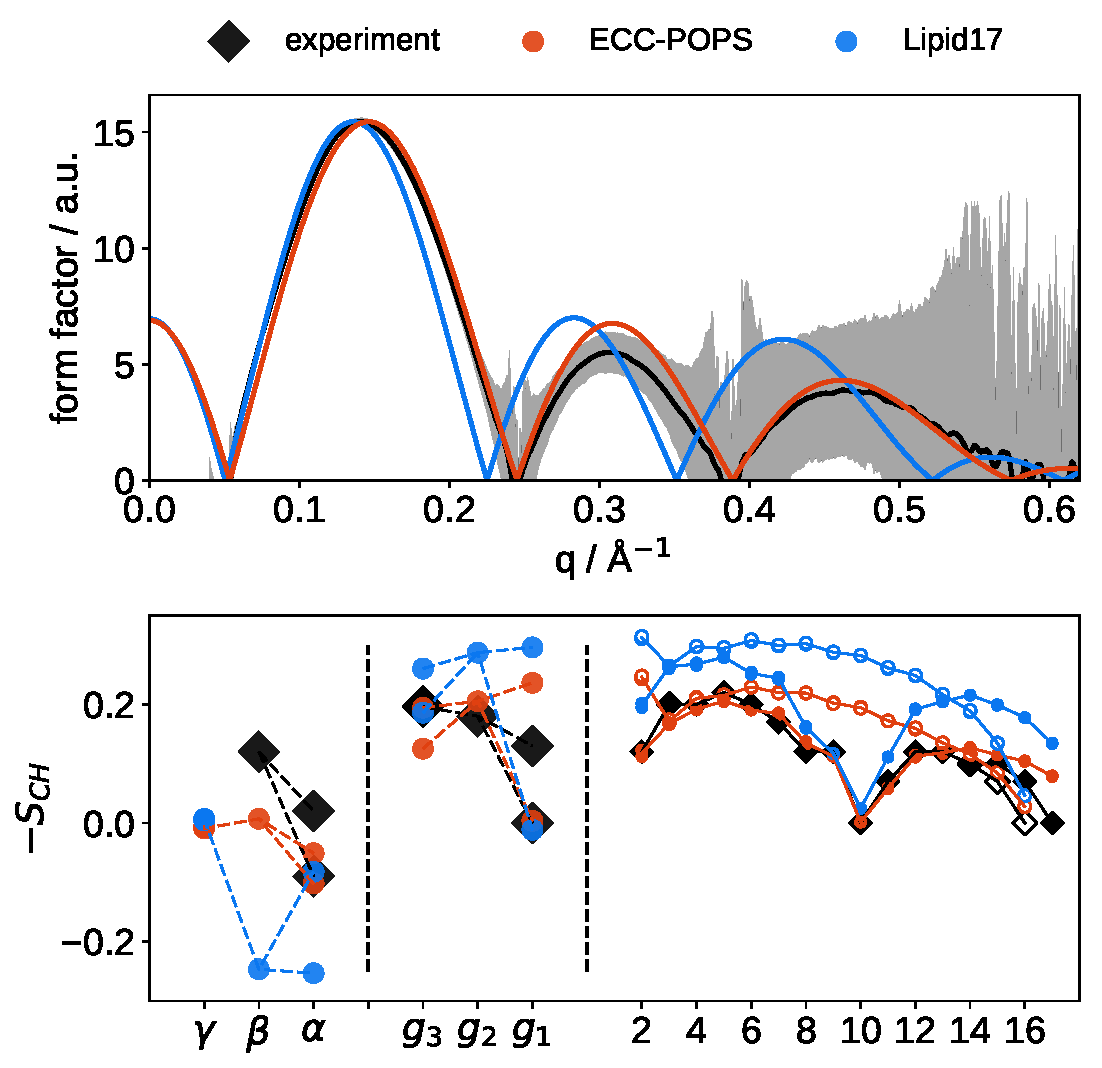
\includegraphics[width=\figwidth]{../img/ecc_pops/Order-parameters_form-factors_exp-L17-ECC-lipids.pdf}
  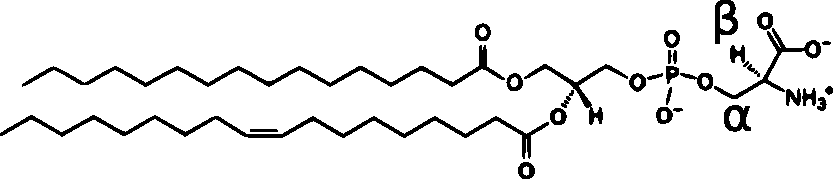
\includegraphics[width=\figwidth]{../img/ecc_pops/pops_chemfig.pdf} 
\hfill
  \caption{\label{simVSexpNOions_POPS} 
    Top: X-ray scattering form factors from simulations with the Lipid17 \citep{lipid17-future} and 
    the ECC-POPS models compared with experiments~\citep{kucerka14} at 298~K. 
    Middle: Order parameters of POPS head group, glycerol backbone and acyl chains  
    from simulations with the Lipid17 \citep{lipid17-future} and the ECC-POPS models 
    compared with experiments at 298~K. \citep{nmrlipids_proj4}
    Open/closed symbols are used for palmitoyl/oleoyl chains of POPS. 
    Bottom: The chemical structure of POPS and the labeling of the carbon segments. 
  }  
\end{figure} 
 


\begin{table}[tb!] 
\centering
  \caption{Values of the area per lipid (APL) of POPS bilayers 
	   at 298~K with only \ce{Na^+} counterions and no additional ions. \label{tab:apls} } 
  \begin{tabular}{l|c c} 
%    \multicolumn{3}{c}{POPC} \\
%    model          & APL / Å$^2$   & $T$ / K  \\ 
%    \hline 
%    Lipid14 POPC \citep{melcr18}    & 65.1$\pm$ 0.6  &  300 \\ 
%    Lipid14 POPC \citep{dickson14}  & 65.6$\pm$ 0.5  &  303 \\ 
%    \hline 
%    ECC-POPC     \citep{melcr18}    & 63.2$\pm$ 0.6  &  300       \\ 
%    \hline 
%    experiment (SDP model) \citep{kucerka11} & 64.3  &  303    \\ 
%    \hline 
%    \multicolumn{3}{c}{} \\
%    \multicolumn{3}{c}{POPE} \\
%    model          & APL / Å$^2$   & $T$ / K  \\ 
%    \hline 
%    ECC-POPE                 & 56.7$\pm$ 0.8  &  298 \\ 
%    \hline 
%    experiment   \citep{parsegian89} & 56.6  &  310    \\ 
%    experiment   \citep{rappolt03}   & 59--61 &  303--313  \\ 
%    \hline 
%    \multicolumn{3}{c}{} \\
    \multicolumn{3}{c}{POPS} \\
    model          & APL / Å$^2$   & $T$ / K  \\ 
    \hline 
    Lipid17 POPS              & 53.5$\pm$ 0.8  &  298 \\ 
    \hline 
    ECC-POPS                & 60.3$\pm$ 0.6  &  298       \\ 
    \hline 
    experiment (SDP model) \citep{kucerka14} & 62.3  &  298    \\ 
    \hline 
  \end{tabular} 
\end{table} 
 
\todo{SAMULI: Lipid17 simulations are too compressed, which is probably due to the
  overbinding of Dang ions. Lipid17 with Åqvist ions (default in Amber) has larger
  area in NMRlipids IV. This is similar to ECC-POPC paper where changing from Åqvist to
  Dang or ECC-ions increased binding affinity in Lipid14. However, the headgroup order
  parameters are better in ECC-POPS compared to Lipid17 simulations with any ions.
  These should be discussed in this section.
}

We compared X-ray scattering form factors and NMR order parameters of bilayers
in pure water without any ions (or only counter ions)
from simulations and experiments
as the first step in the assessment of the quality of the model. 
The experimental X-ray scattering form factors 
of a bilayer are well reproduced  
(see Fig.~\ref{simVSexpNOions_POPS}). 

The area per lipid is often used as a relatively simple structural parameter reporting on the bilayer properties and the packing of lipids. 
In experiments, modeling is used on top of the scattering factors to obtain it \citep{kucerka14}. 
From simulations, this property is easily extracted. 
We compare the values from experiments and simulations in Table~\ref{tab:apls}. 


While the agreement between the scattering form factors 
from the simulation of a pure POPS bilayer and experiment 
are excellent (Fig.~\ref{simVSexpNOions_POPS}),
there is a non-negligible difference between the values of the area per lipid in Table~\ref{tab:apls}. 
Since both values are derived from the scattering form factors through modeling of the electron density of the bilayer,
we cannot decide, which of the values is more reliable. 
In general, we can conclude that ECC-lipids
%the presented lipid models with ECC-lipids 
reproduce the experimental structural parameters of the lipid bilayers 
with a comparable accuracy to existing state-of-the-art lipid models~\citep{botan15, ollila16, Pluhackova2016}. 
 
The head group and acyl chain order parameters within ECC-lipids
are in general in a good agreement with the experimental values 
as shown in Fig. \ref{simVSexpNOions_POPS}. 
The acyl chain order parameters in particular are almost all within the experimental error bars.
The order parameters of the head groups are at an accuracy comparable to 
other currently available classical models of lipids \citep{botan15, catte16, Pluhackova2016}. 

The head group order parameters $\alpha$ and $\beta$ are highly relevant for this work,
as they are being used in the electrometer concept \cite{altenbach84, catte16, melcr18}.
For POPC in pure water, the order parameter $\beta$ agrees well with the experiment, 
while the order parameter $\alpha$ is somewhat lower. 
In the case of POPS, the situation is a bit more complicated
compared to POPC as the order parameter $\alpha$ exhibits a notable forking (see Fig.~\ref{simVSexpNOions_POPS}).
One of the order parameters of ECC-POPS, $\alpha_1$, agrees well with the experiment, 
while the other, $\alpha_2$, adopts a higher value underestimating the experimentally reported forking. 
There is only one order parameter $\beta$ in POPS, 
which has a higher value closer to zero in the ECC-lipids model than in experiment. 
Such a feature suggests that the model overestimates the orientational freedom of its head group. 

 
 
 
\subsection{Interactions between PC and PS head groups in mixed PC:PS bilayers}


Changes of the lipid bilayer head group order parameters extracted from simulations and 
experiments \cite{roux90} are shown in Figs.~\ref{fig:delta_ordPar_KCl_PCPS}, \ref{fig:delta_ordPar_NaCl_PCPS} 
and~\ref{fig:delta_ordPar_CaC_PCPS} as functions of KCl, NaCl or CaCl$_2$ concentrations,
and in Figs.~\ref{fig:delta_ordPar_NaCl_PC-PS_mix} as a function of PC and PS content. 



\begin{figure*}[!htb] 
  \centering 
  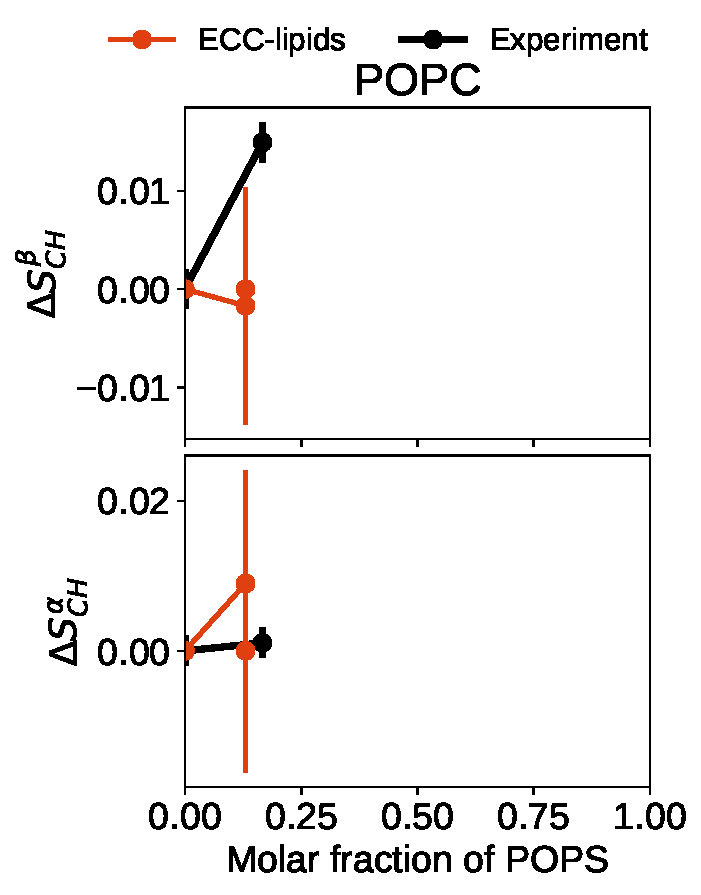
\includegraphics[width=\figwidthsmall]{../Fig/order_parameters_changes_A-B_PC-PS_mix_POPC_nacl.pdf} 
  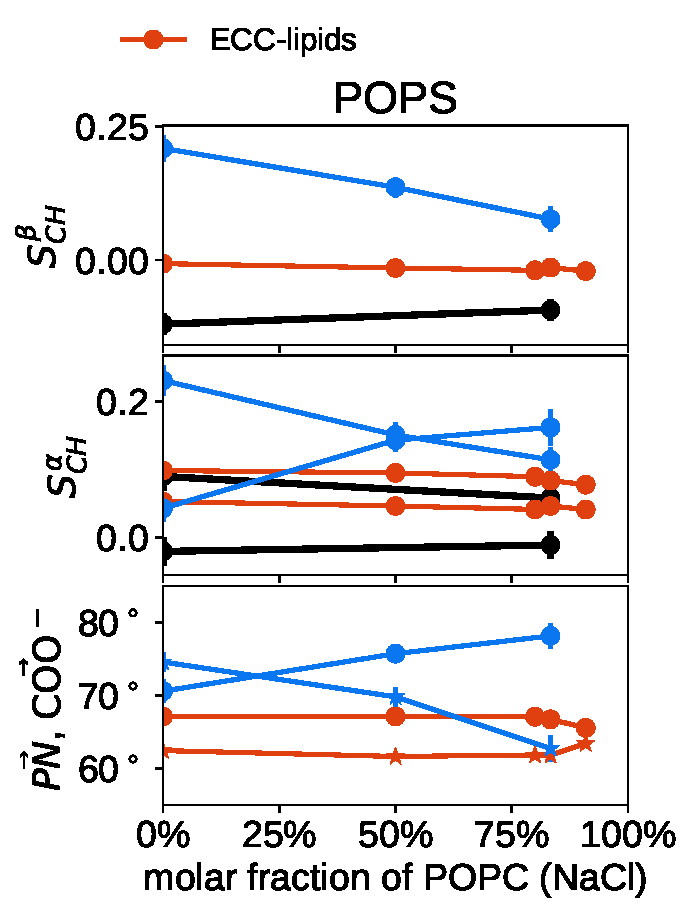
\includegraphics[width=\figwidthsmall]{../Fig/order_parameters_changes_A-B_PC-PS_mix_POPS_nacl.pdf} 
  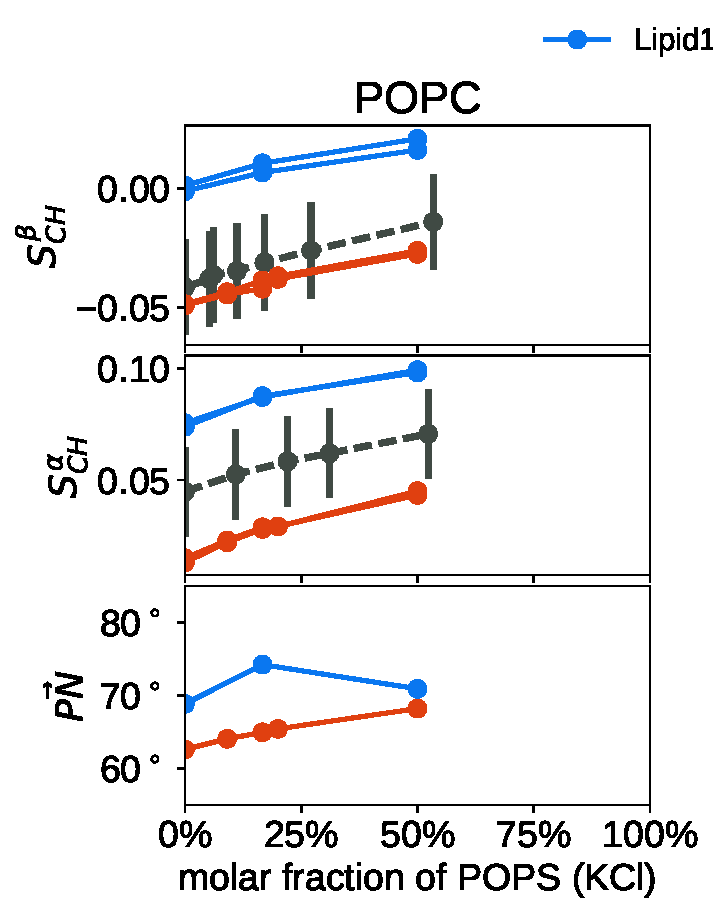
\includegraphics[width=\figwidthsmall]{../Fig/order_parameters_changes_A-B_PC-PS_mix_POPC_kcl.pdf} 
  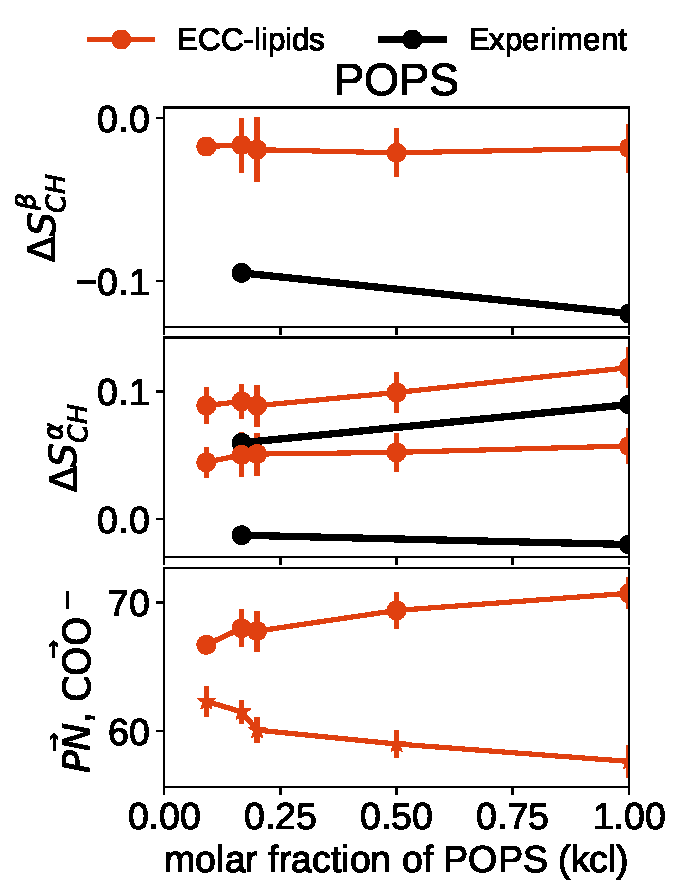
\includegraphics[width=\figwidthsmall]{../Fig/order_parameters_changes_A-B_PC-PS_mix_POPS_kcl.pdf} 
  \caption{\label{fig:delta_ordPar_NaCl_PC-PS_mix} 
    Changes of the head group order parameters of a POPC:POPS (5:1) bilayer as a function of PS content
    with \ce{Na^+} and \ce{K^+} counterions from simulations with ECC-lipids and Lipid17 \cite{lipid17-future} 
    and experiments (only \ce{Na^+} counterions). \cite{roux90}. 
    The underestimated response of ECC-lipids with \ce{Na^+} counterions 
    is likely due to a still slightly overestimated binding affinity of \ce{Na^+} to the phospholipids,
    which is corroborated by the series with \ce{K^+} counterions (lower affinity than \ce{Na^+}),
    where the response is closer to the experiment (which uses only \ce{Na^+} counterions). 
    Experimental points for POPS inherently contain larger systematic error, 
    as they come from independent experiments.
  }
  \todo{SAMULI: Caption says Åqvist, but I guess that Dang is used also here?} \\
  \todo{SAMULI: Do you have a simulation of Lipid14 pure POPC at 298K?
    This is not in the table. This simulation would be useful also for NMRlipids IV.
  } \\
  \todo{SAMULI: Error bars for lipid14 missing.}
\end{figure*} 




 
 
 


\subsection{Molecular interaction and binding affinities of K$^+$ and Na$^+$ cations to mixed POPC:POPS (5:1) membrane} 
\label{sec:affinity} 

 
 
\begin{figure}[tbp!] 
  \centering 
  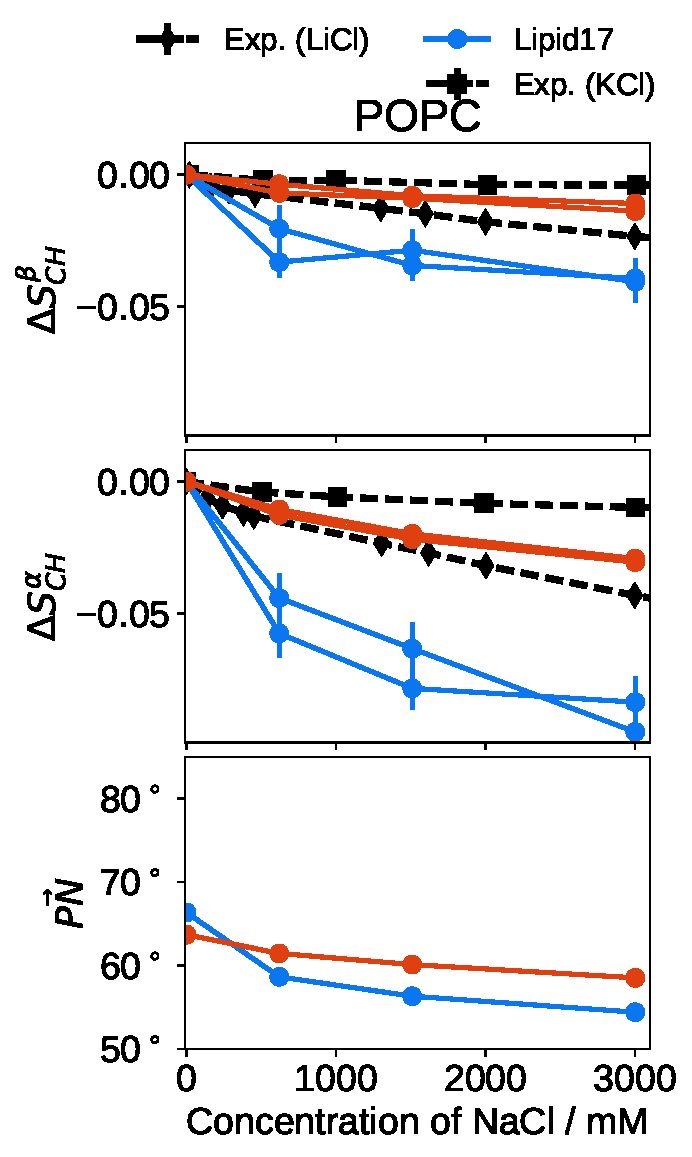
\includegraphics[width=\figwidthsmall]{../img/ecc_pops/order_parameters_changes_ecc-lip_L14_A-B-PN-COO_POPC_nacl.pdf} 
  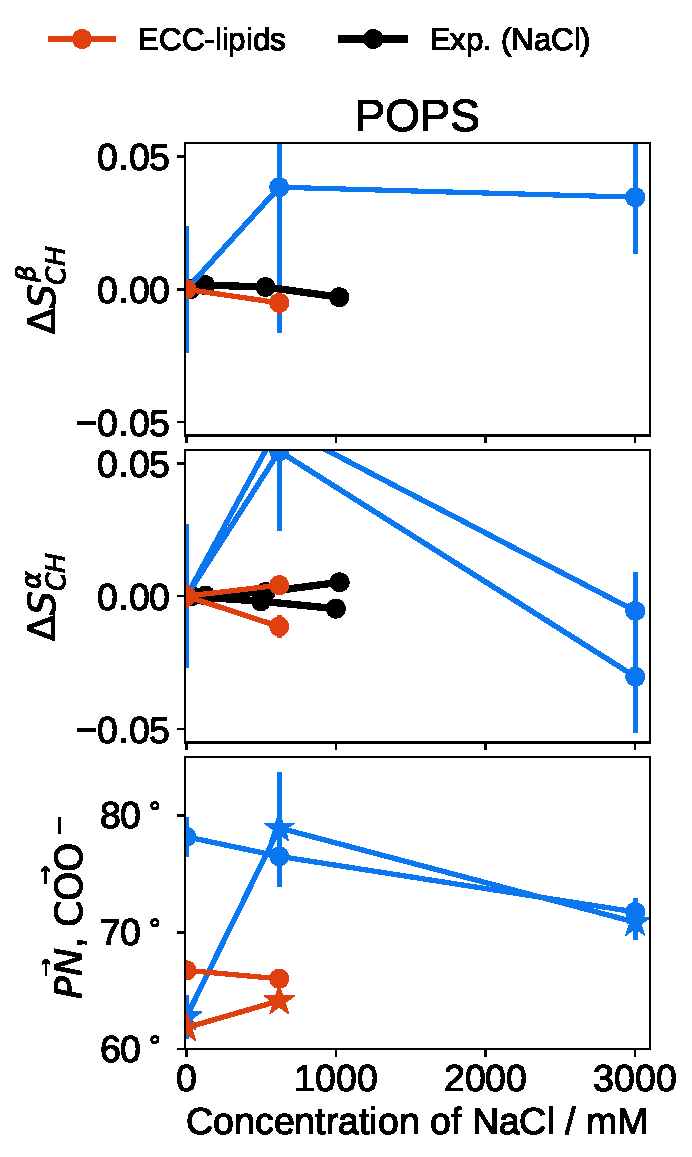
\includegraphics[width=\figwidthsmall]{../img/ecc_pops/order_parameters_changes_ecc-lip_L14_A-B-PN-COO_POPS_nacl.pdf} 
  \caption{\label{fig:delta_ordPar_NaCl_PCPS} 
    Changes of the head group order parameters $\alpha$, $\beta$ and the orientations of the carboxylate group and the P-N vector  
    of POPC (left) and POPS (right) phospholipids in a POPC:POPS 5:1 bilayer as a function of \ce{NaCl} concentration 
    in bulk ($C_{ion}$) from simulations with different force fields at 298 K.
    Because data with \ce{NaCl} are not available for POPC, 
    we show experimental data for \ce{LiCl} (dashed line, left) 
    as an upper bound for the magnitude of the response to \ce{NaCl}, 
    which has a lower affinity to phospholipid bilayers compared to \ce{LiCl} \citep{roux90}. 
    The orientation of the \ce{COO^-} group is defined as 
    the connector from the $\beta$ carbon to the carbon in \ce{COO^-} (stars, bottom right). 
  } 
  \todo{SAMULI: The forking of PS alpha carbon should not be put to zero with zero salt concentrations
    in this or in other figures. This is confusing expecially for the results with CaCl$_2$ where the forking
    seems to increase with CaCl$_2$, which is not correct. In NMRlipids IV, I have now put the lower order parameter
    to zero and kept the forking correct with all concentrations of ions.} \\
  \todo{SAMULI: Ion concentrations should be updated to the concentrations in water before solvating the lipids.} \\
  \todo{SAMULI: Error bars should be recalculated with the fixed code} \\
  \todo{SAMULI: We should have at least one more points with higher concentration (maybe close to 2M), or maybe two more points.} \\
  \end{figure} 


\begin{figure}[tbp!] 
  \centering 
  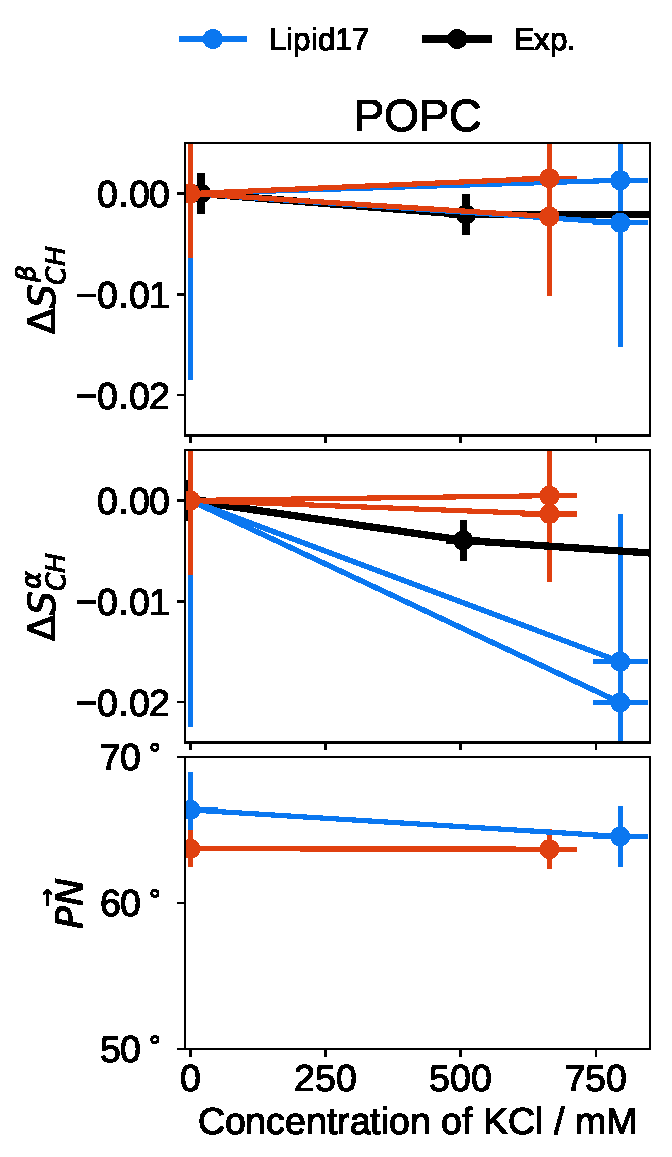
\includegraphics[width=\figwidthsmall]{../img/ecc_pops/order_parameters_changes_ecc-lip_L14_A-B-PN-COO_POPC_kcl.pdf} 
  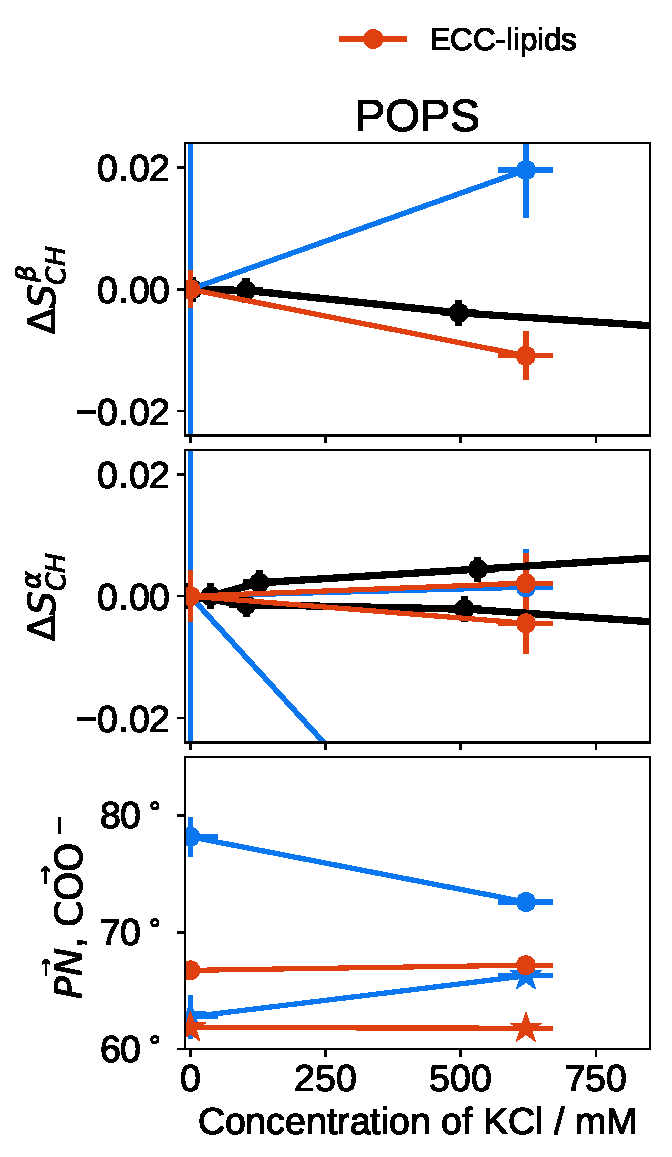
\includegraphics[width=\figwidthsmall]{../img/ecc_pops/order_parameters_changes_ecc-lip_L14_A-B-PN-COO_POPS_kcl.pdf} 
  \caption{\label{fig:delta_ordPar_KCl_PCPS} 
    Changes of the head group order parameters $\alpha$, $\beta$ and the orientations of the carboxylate group and the P-N vector  
    of POPC (left) and POPS (right) phospholipids in a POPC:POPS 5:1 bilayer as a function of \ce{KCl} concentration 
    in bulk ($C_{ion}$) from simulations with different force fields and experiments at 298 K. \citep{roux90}
    The orientation of the \ce{COO^-} group is defined as 
    the connector from the $\beta$ carbon to the carbon in \ce{COO^-} (stars, bottom right). 
  } 
  \todo{SAMULI: The forking of PS alpha carbon should not be put to zero with zero salt concentrations
    in this or in other figures. This is confusing expecially for the results with CaCl$_2$ where the forking
    seems to increase with CaCl$_2$, which is not correct. In NMRlipids IV, I have now put the lower order parameter
    to zero and kept the forking correct with all concentrations of ions.} \\              
  \todo{SAMULI: Ion concentrations should be updated to the concentrations in water before solvating the lipids.} \\
  \todo{SAMULI: Error bars should be recalculated with the fixed code} \\
  \todo{SAMULI: We should have at least one more points with higher concentration (maybe close to 2M), or maybe two more points.} \\
\end{figure} 
 


% Pavel suggested to remove this as it only recaps previous sections
%It was presented in the previous section,
%that accounting for electronic polarization,
%a distinct feature of ECC-lipids compared to other lipid models, 
%is crucial for an accurate description of the response of the POPC electrometer. 
%In this section,
%we employ ECC-lipids to simulate neutral and negatively charged bilayers 
%in the presence of monovalent salts, namely \ce{KCl} and \ce{NaCl}. 

The binding of \ce{Na^+} cations to phospholipid bilayers 
is not generally agreed on between simulations 
\citep{bockmann03,sachs04,berkowitz06,cordomi09}
and experiments 
\citep{cevc90,tocanne90,hauser76,herbette84,uhrikova08}.
We attempted to find a model, 
which would successfully interpret the experiments on binding of \ce{Na^+}
to neutral and negatively charged phospholipid bilayers \citep{akutsu81, roux90} 
in our works \citep{catte16, nmrlipids_proj4}.
After testing the currently available force fields for phospholipids,
we concluded
that the interactions are generally overestimated in magnitude in almost all models 
but Lipid14 (PC) \citep{dickson14}, resp. Lipid17 (PS) \citep{lipid17-future}. 
This model yields a semi-quantitative agreement with the experimentally measured small changes of the order parameters 
when used with the model of ions by \citet{aqvist90} (Fig.~\ref{fig:catte16}). 
However, when used with a more accurate model of ions by \citet{Pluharova2014, martinek17},
the model overestimates the binding affinity of \ce{Na^+}
measured with lipid electrometer concept. \citep{melcr18}
In total, these results suggest that improvements 
in the lipid parameters are required for more accurate interactions even with monovalent cations. 
\citep{catte16, melcr18, nmrlipids_proj4}

Generally improved behaviour 
of the POPC and POPS head group order parameters 
with \ce{NaCl} or \ce{KCl} concentrations 
was achieved through the combination of models 
ECC-lipids \citep{melcr18} and ECC-ions \citep{martinek17, kohagen16, Pluharova2014}. 
Simulations with these models 
reveal a good agreement with the NMR experiments 
for both neutral and negatively charged membranes.
The results are plotted for \ce{NaCl} in Fig. \ref{fig:delta_ordPar_NaCl_PCPS}, 
and for \ce{KCl} in Fig. \ref{fig:delta_ordPar_KCl_PCPS}. 


The interaction with \ce{K^+}, which binds very weakly to both neutral and negatively charged membranes, 
renders a qualitatively different response of the order parameter $S^\beta$ in POPS in the mixed negatively charged bilayers compared to the neutral bilayers. 
While the order parameter $S^\beta$ increases for both \ce{Na^+} and \ce{Ca^{2+}},
it decreases in the presence of \ce{K^+}.
%This feature is, \emph{qualitatively} captured by a few models in \citep{nmrlipids_proj4},
%neither of them is as close to a \emph{qunatitative} agreement with the experiments 
%as the combination of ECC-lipids with ECC-ions. 
However, no model studied in \citep{nmrlipids_proj4} describes the behaviour of a PS head group correctly enough to reveal this effect. 
In contrast, ECC-lipids with ECC-ions capture the different response of the order parameters $S^{\beta}$, $S^{\alpha _1}$ and $S^{\alpha _2}$ in POPS to various salts accurately. 
Such a detailed description of the changes of the structural parameters 
demonstrates that including electronic polarization
improves the description of the interactions even for very weakly binding cations like \ce{K^+}. 




\begin{figure}[tbp!] 
  \centering 
  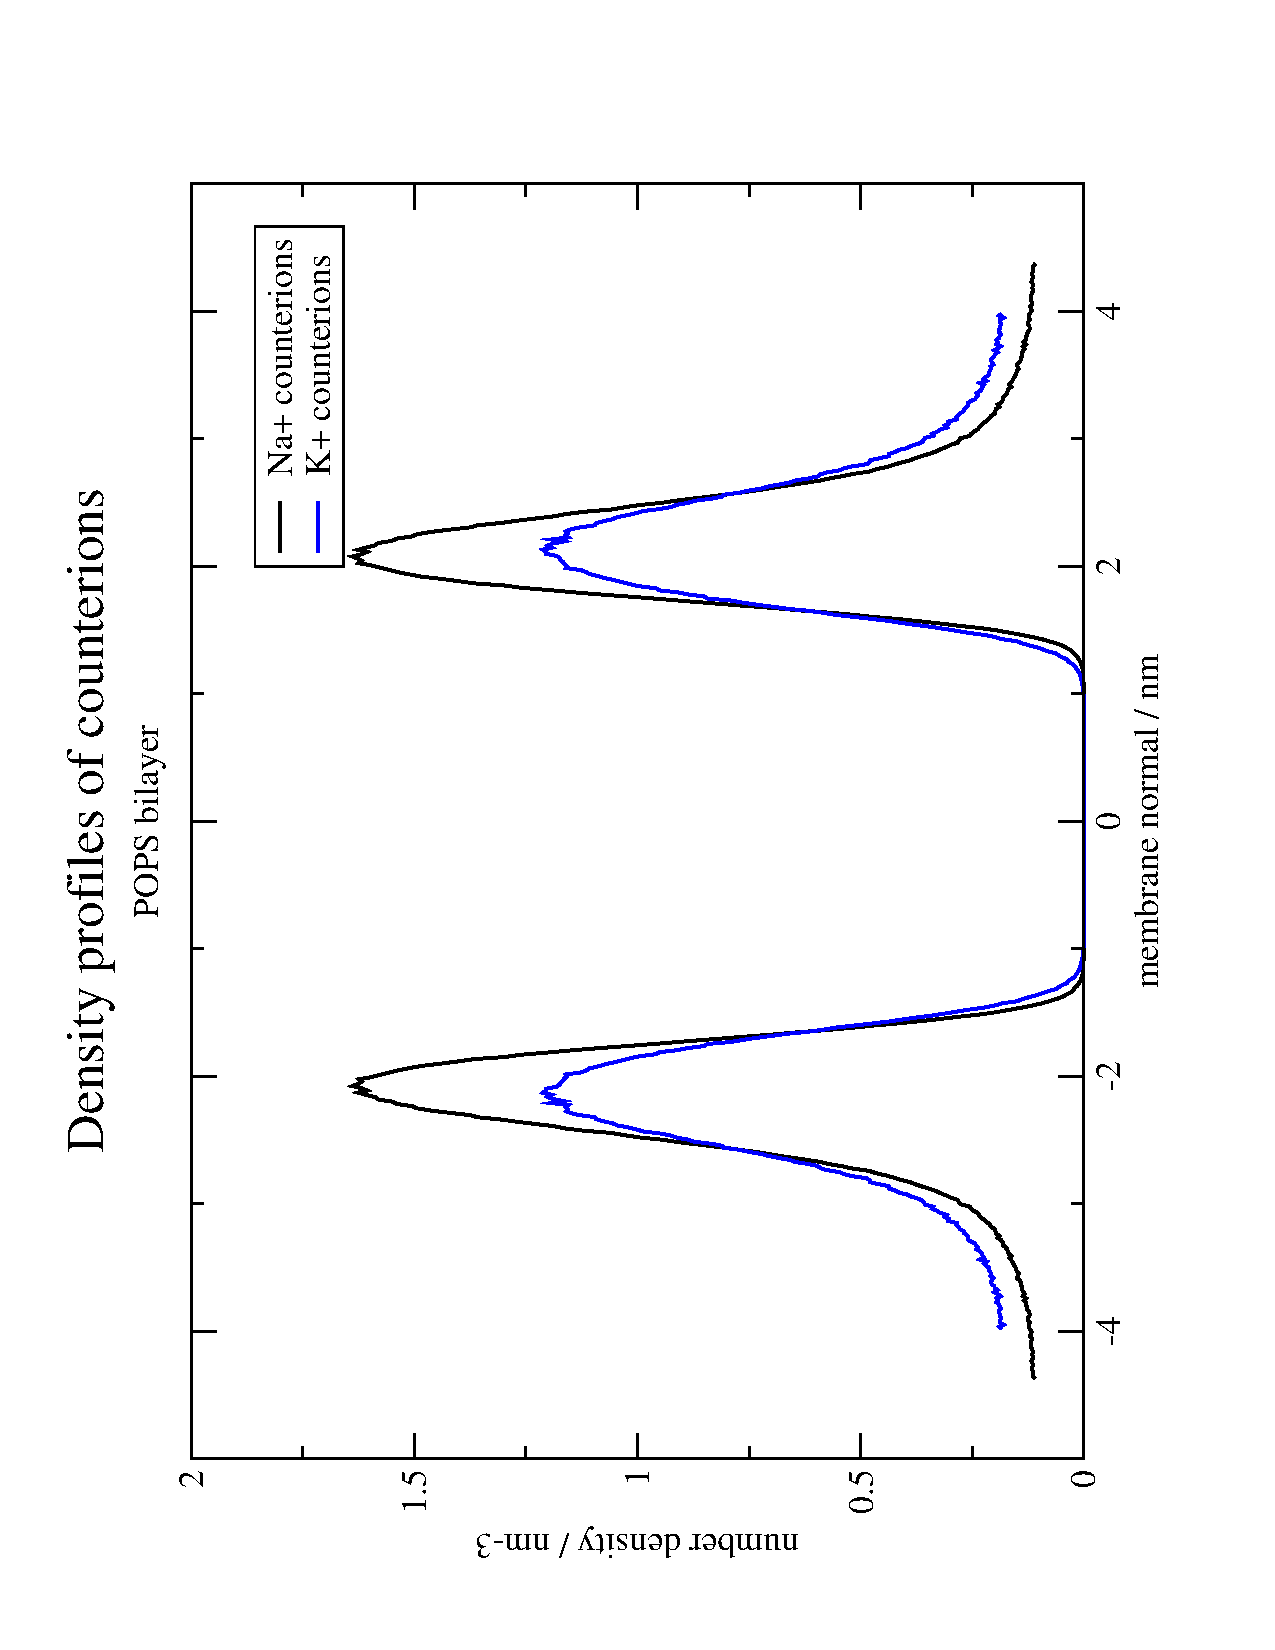
\includegraphics[width=\figwidth]{../img/density_profile_K-Na_counterions_compar_pure-ECC-POPS.pdf}
  \caption{\label{fig:POPS-counterions-dens}
    Number density profiles of \ce{K^{+}}, \ce{Na^{+}} counterions along the membrane normal axis 
    for the negatively charged POPS bilayers using ECC-lipids and ECC-ions.  }
\todo{Joe: TO BE UPDATED + results from PC:PS mixutres to be added.}
\end{figure} 


\begin{figure}[tbp!] 
  \centering 
  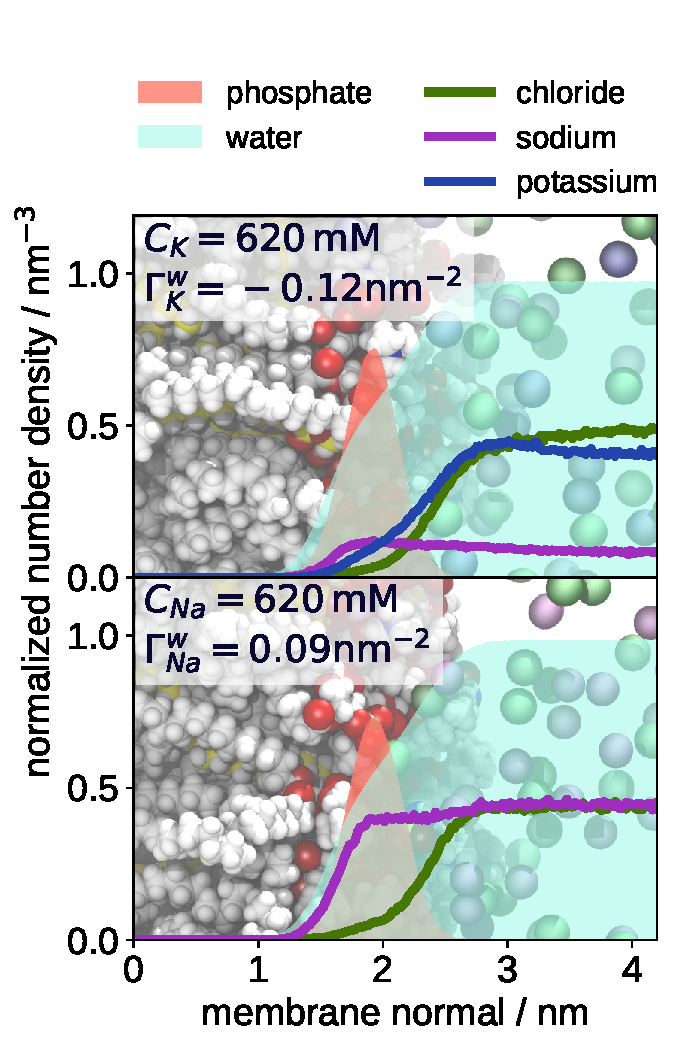
\includegraphics[width=\figwidth]{../img/ecc_pops/density_profiles_na_k_cl_wat_phos_models-compar_5-6_NaCl-and-KCl-series.pdf}
  \caption{\label{fig:nacl-dens_PCPS} 
    Number density profiles of \ce{K^{+}}, \ce{Na^{+}} and \ce{Cl^-} along the membrane normal axis 
    for the negatively charged membranes with the composition of 5\,PC:1\,PS using ECC-lipids and ECC-ions
    from simulations with added concentrations of \ce{KCl} or \ce{NaCl}.  
    The top    profile shows the simulation with an additional \ce{KCl} concentration and \ce{Na^+} counterions. 
    The bottom profile shows the simulation with an additional \ce{NaCl} concentration and \ce{Na^+} counterions, which are not distinguished from the added salt. 
    The density profiles of phosphate groups and water are divided by 4 and 100, respectively.  
  }
\end{figure} 



The difference between the affinities of \ce{Na^+} and \ce{K^+} to neutral and negatively charged membranes
can be described by their relative surface excesses with respect to water, $\Gamma ^{w} _{ion}$, 
which are shown in the plots of the density profiles of the ions in Figs.~\ref{fig:nacl-dens} (neutral bilayer)
\todo{SAMULI: We should have a figure showing density profiles of Na+ and K+ in pure POPS and PC:PS (5:1) mixture
  with only counterions from ECC-POPS model and Lipid17 model.
}
and \ref{fig:nacl-dens_PCPS} (negatively charged bilayer). 
Such a quantity compares the adsorption of ions to the adsorption of water molecules at an interface 
without the necessity of defining a Gibbs dividing surface. \citep{melcr18, chattorajBOOK}
While \ce{K^+} maintains negative values of $\Gamma^{w}_{K}$ even for the negatively charged bilayer,
the value of $\Gamma^{w}_{Na}$ for \ce{Na^+} changes from negative to positive
in a neutral POPC bilayer versus in a negatively charged bilayer with the composition 5\,PC:1\,PS.
%This means that at the given concentration the bilayer interface has a small preference to \ce{Na^+} cations compared to water molecules. 
Interestingly, this value is slightly decreased in the presence of an additional \ce{NaCl} concentration adding also \ce{Cl^-} anions, 
which are not present in the system when only counterions are used
(bottom resp. top plot in Fig.~\ref{fig:nacl-dens_PCPS}). 
The relative surface excess of calcium, $\Gamma^{w}_{Ca}$, also reflects
the higher affinity of the negatively charged PC:PS (5:1) membrane compared to a neutral POPC bilayer; 
its value for the latter is       $\Gamma^{w}_{Ca} = 0.06\mathrm{nm^{-2}}$, 
while for the PC:PS mixture it is $\Gamma^{w}_{Ca} = 0.24\mathrm{nm^{-2}}$
at comparable concentrations $C _{Ca} = 260\pm 30 \mathrm{mM} $. 


 





 
 


\subsection{Molecular interaction and binding affinities of \ce{Ca^{2+}} cations to mixed POPC:POPS (5:1) membrane} 
\label{section:lip-ion_ca}



\begin{figure}[tbp!] 
  \centering 
  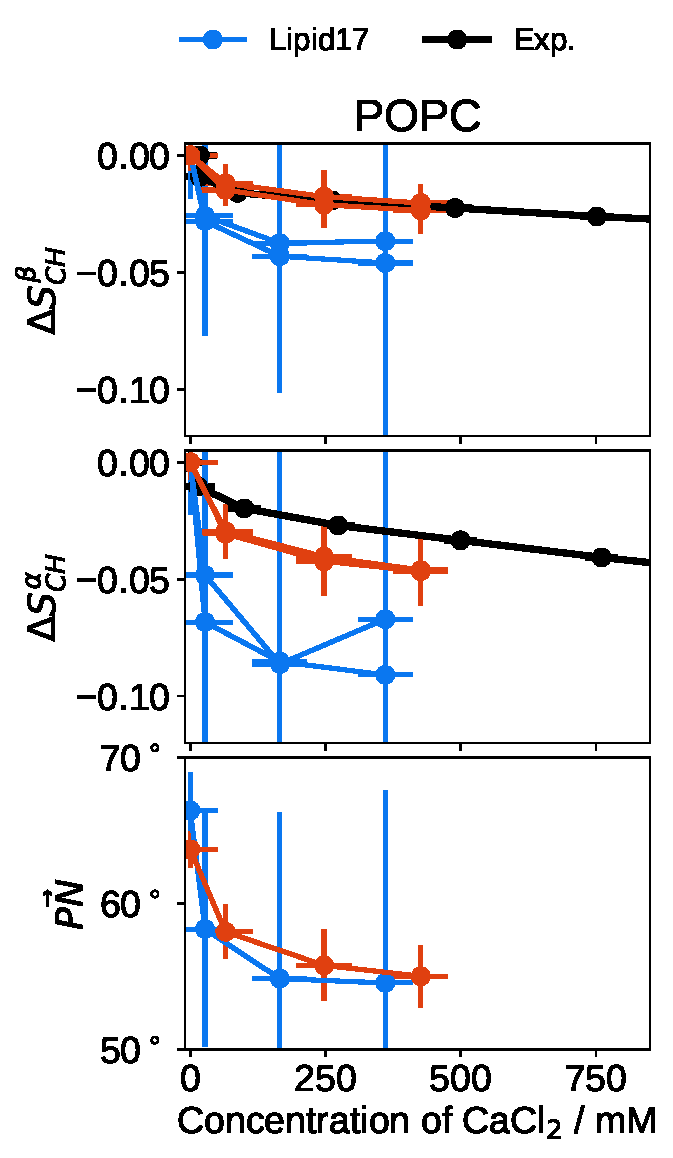
\includegraphics[width=\figwidthsmall]{../img/ecc_pops/order_parameters_changes_ecc-lip_L14_A-B-PN-COO_POPC_cacl.pdf} 
  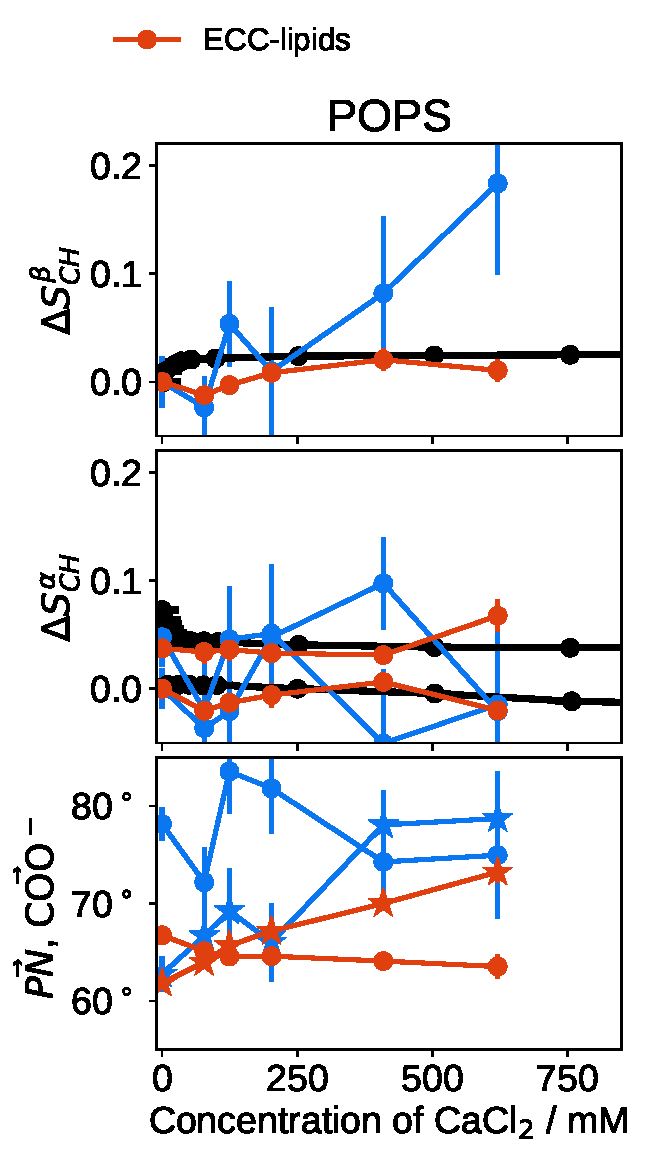
\includegraphics[width=\figwidthsmall]{../img/ecc_pops/order_parameters_changes_ecc-lip_L14_A-B-PN-COO_POPS_cacl.pdf} 
  \caption{\label{fig:delta_ordPar_CaCl_PCPS} 
    Changes of the head group order parameters $\alpha$, $\beta$ and the orientations of the carboxylate group and the P-N vector  
    of POPC (left) and POPS (right) phospholipids in a POPC:POPS 5:1 bilayer as a function of \ce{CaCl2} concentration 
    in bulk ($C_{ion}$) from simulations with different force fields and experiments at 298~K. \citep{roux90}
    The orientation of the \ce{COO^-} group is defined as 
    the connector from the $\beta$ carbon to the carbon in \ce{COO^-} (stars, bottom right). 
  } 
  \todo{SAMULI: The forking of PS alpha carbon should not be put to zero with zero salt concentrations
    in this or in other figures. This is confusing expecially for the results with CaCl$_2$ where the forking
    seems to increase with CaCl$_2$, which is not correct. In NMRlipids IV, I have now put the lower order parameter
    to zero and kept the forking correct with all concentrations of ions.} \\
  \todo{SAMULI: Ion concentrations should be updated to the concentrations in water before solvating the lipids.} \\
  \todo{SAMULI: Error bars should be recalculated with the fixed code} \\
  \todo{SAMULI: Maybe we should have at least one more points with smaller concentration
    (maybe close to 100mM in solution before solvating lipids).} \\
\end{figure} 



%%% Sum up what is to be presented briefly
%The importance of treating polarizability for interactions of phospholipids with monovalent ions was demonstrated in the previous section. 
Electronic polarization is a non-negligible contribution to the interactions of calcium even in simple aqueous solutions of \ce{CaCl2} \citep{martinek17, kohagen16, Pluharova2014}. 
In this section,
we will show the results from simulations of neutral and negatively charged phospholipid bilayers at varying \ce{CaCl2} concentrations
using the recently developed models ECC-lipids and ECC-ions \citep{melcr18, martinek17}, 
which implicitly include the effects of electronic polarization through electronic continuum correction \citep{leontyev11}. 
Validated with the concept of a lipid electrometer in section \ref{section:electrometer_exp_sim},
these implicitly polarizable models yield accurate description of 
the interaction of \ce{Ca^{2+}} with both neutral and negatively charged phospholipids. 

The changes of the head group order parameters $S^\alpha$ and $S^\beta$ from simulations and experiments 
are shown in Fig.~\ref{fig:delta_ordPar_CaCl} for a neutral POPC bilayer, 
and in Fig.~\ref{fig:delta_ordPar_CaCl_PCPS} for a negatively charged bilayer with the composition 5\,PC:1\,PS. 
For a direct comparison and a connection to our works \citep{catte16, nmrlipids_proj4},
we show simulation results from ECC-lipids and also from Lipid17 \citep{lipid17-future}. 
This also highlights the improvements in ECC-lipids over Lipid17 arising from the electronic polarization. 
%Although Lipid17 already belongs to the top-performing models in terms of the responses of the head group order parameters in those studies,  
%including electronic polarizability to form ECC-lipids improves the results even further.
The effect is probably the most striking for POPS, 
for which also the structure of a pure POPS bilayer with only counterions is dramatically improved with the augmentation. 


%%% Discuss the changes of OPs and vectors from neutral and neg. membranes
%While the changes induced by \ce{CaCl2} are \emph{qualitatively} correct for Lipid14/17, 
Increasing concentrations of \ce{CaCl2} induce a systematic decrease of the order parameters $S^\alpha$ and $S^\beta$ in POPC. 
Although the total magnitude of the response of the PC head group order parameters 
is only slightly higher in the negatively charged bilayers than in the neutral bilayers, 
the shape of the changes in the latter shows a steeper onset at low concentrations. 
This is apparently due to the presence of POPS, 
which has a higher affinity to \ce{Ca^{2+}} compared to POPC. 
ECC-lipids is the first model,
which achieves a \emph{quantitative} agreement with the changes induced by \ce{CaCl2} in experiments. 

\todo{SAMULI: The qualitative iprovement of PS headgroup order parameter response to bound Ca2+
  should be discussed. We should, however, point out that the response PS alpha carbon to bound
  Ca2+ is not excatly reproduced even by the ECC-POPS model.
}




\begin{figure}[htbp!] 
  \centering 
  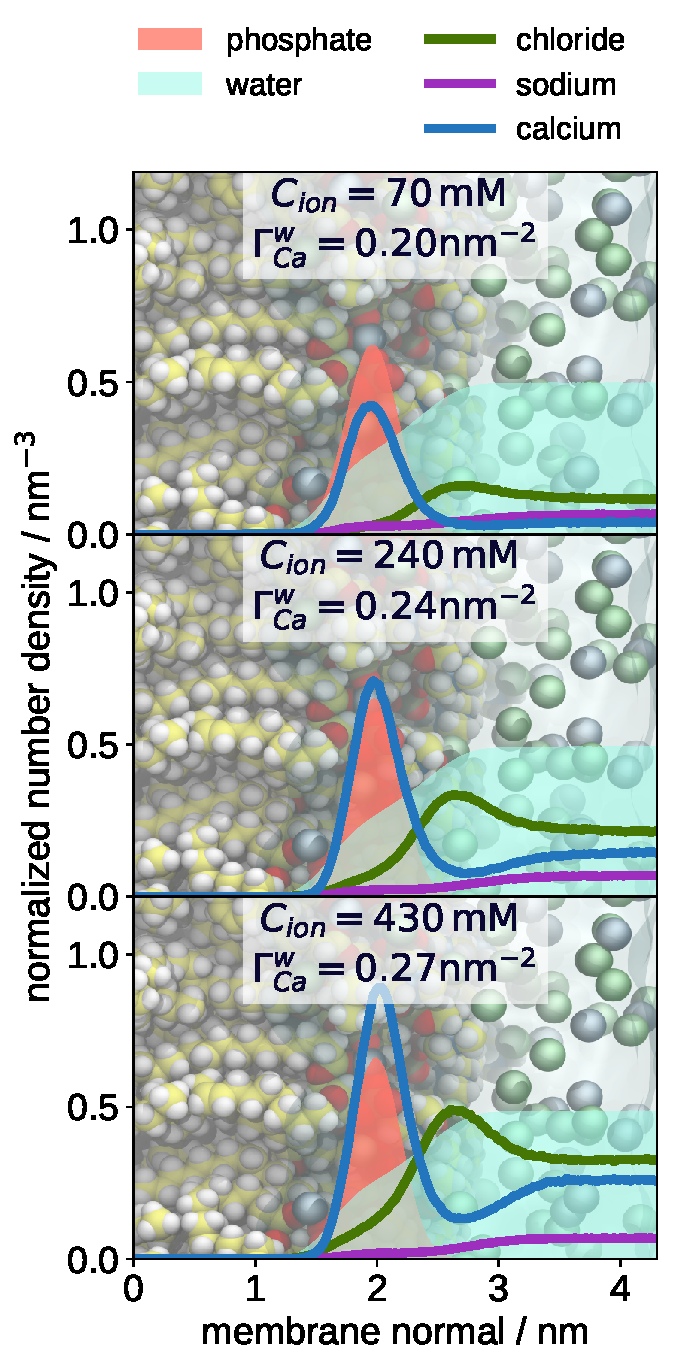
\includegraphics[width=\figwidth]{../img/ecc_pops/density_profiles_ca_na_cl_wat_phos_models-compar_1-3_CaCl2-series.pdf}
  \caption{\label{fig:cacl-dens_PCPS} 
    Number density profiles of \ce{Ca^{2+}}, \ce{Na^{+}} and \ce{Cl^-} along the normal of the membrane starting at the centre
    for the negatively charged membrane with the composition 5\,PC:1\,PS
    at various bulk concentrations of \ce{CaCl2} from simulations with ECC-lipids. 
    All profiles contain \ce{Na^+} counterions and an additional concentration of \ce{CaCl2}. 
    In order to visualize the density profiles with a scale comparable to the profile of \ce{Ca^{2+}},  
    the density profiles of~\ce{Cl^-} ions are divided by 2, and 
    the density profiles of phosphate groups and water are divided by 5 and 200, respectively.  
  }
  \todo{SAMULI: Ion concentrations should be updated to the concentrations in water before solvating the lipids.} \\
  \todo{SAMULI: We should compare to the density profiles from Lipid17 simulations. These are also needed for NMRlipids IV.}
\end{figure} 
 





%%% Present the density profiles (different concentrations for both POPC and mixed)
The increase in the amount of bound calcium cations from pure POPC \cite{melcr18}
to the mixed negatively charged bilayer containing POPS
is well demonstrated using the relative surface excess, $\Gamma ^w _{Ca}$,
summarized in Table~\ref{tab:binding}. 
Distributions of \ce{Ca^{2+}}, \ce{Na^+} counterions and also \ce{Cl^-} 
are plotted in Fig.~\ref{fig:cacl-dens_PCPS} for the negatively charged bilayer. 
In contrast to \ce{KCl} or added concentrations of \ce{NaCl}, 
\ce{Na^+} counterions are substituted with \ce{Ca^{2+}} even at low concentrations of \ce{CaCl2}. 
The increasing concentration of \ce{CaCl2} and, hence, a higher amount of bound \ce{Ca^{2+}}
also attracts \ce{Cl^-} anions to the bilayer 
as can be seen from its growing density at the interface. 

\todo{SAMULI: This paragraph in unclear. Should be clarified and the changes
  of headgroup orientations in PC and PS clearly discussed.
}
%%% discuss the table with Gammas and follow up with molecular details, where do cations bind? Support with the spatial density figure
The density profiles of ions suggest that
the dominant contribution to the binding of \ce{Ca^{2+}} to phospholipid bilayers
comes from the interactions with the phosphate groups in both POPC and POPS. 
%The population analysis also suggests 
%that the calcium cations prefer to reside in the phosphate region of the membrane. 
%Such a finding is further validated with a more detailed analysis using Markov state modeling (MSM) \citep{Pande_MSM_paper} \todoi{Add papers reviewing MSM, e.g. recent Pande's paper.}. 
%The set of states of a calcium cation 
%encompassed all possible combinations of up to three surrounding lipids. 
%In the case of PC, we used only the phosphate moitety, which forms the dominant contribution for calcium binding.
%For PS we also distinguished configurations in which calcium interacts with the carboxylate moiety. 
%All possible combinations of such states were used to build a Markov model at a lag time $25\,\mathrm{ns}$ using pyEMMA code by \citet{pyemma} \todoi{add citation for pyemma}. 
%The resulting MSM was validated using Chapman-Kolmogorov test \citep{FrankNoe_papers_MSM} \todoi{Add citation for Noe's papers on MSM, especially Chapman Kolmogorov test.}. 
%The stationary distribution of the states reveals a strong preference of the calcium cations to reside in the phosphate region of the mixed PC-PS membrane. 
%When interacting with PS, configurations with the phosphate moiety from either PC or PS dominate the population.
%Moreover, states containing interactions with the carboxylate group in PS 
%bear higher probability when interacting also with the phosphate group of the same lipid or other lipids. 
This is also reflected in the shift of the mean orientation 
of the \ce{COO^-} group from $62^\circ$ to $73^\circ$ (420~mM \ce{CaCl2})
which was measured as the connector of the carbon atoms 
forming the bond between the group and the $\beta$-carbon of the phospholipid. 
The interactions of the carboxylate group in PS with calcium and other phosphate groups
shed light into the qualitatively different response of the head group order parameters $\alpha$ and $\beta$ in PS compared to PC 
(see Figs.~\ref{fig:delta_ordPar_CaCl} and~\ref{fig:delta_ordPar_CaCl_PCPS}). 
We find that the complex response of the head group order parameters of POPS 
is affected by the conformational changes of the carboxylate group,
which is attracted more towards the phosphate region, 
where the calcium cations dominantly bind. 
In line with the experimental work by \citet{browning80},
this is also very likely the reason, 
why the magnitude of the P-N vector change in POPS is diminished compared to POPC, 
which is not restrained by an additional cation binding group like \ce{COO^-} in POPS. 


Further details about the interactions of \ce{Ca^{2+}} with various moieties in POPC or POPS
were obtained by counting contacts between the cations and the oxygen atoms of the lipids
similarly as was done in \cite{melcr18}. 
The threshold for counting a contact was set to $0.3\,\mathrm{nm}$, 
which encompasses the first peak of the radial distribution function between the cations and the oxygen atoms of the lipids. 


\begin{table}[tb!] 
\centering
  \caption{Bulk concentrations, $C _{Ca}$, and molar fractions, $C' _{Ca}$, of Ca$^{2+}$;
           relative surface excess of calcium with respect to water ($\Gamma_{Ca}^{\rm water}$); 
           and percentages of the population 
           of bound Ca$^{2+}$ to various moieties 
           in a neutral membrane composed of POPC
           and in a negatively charged membrane with the composition 5\,PC:1\,PS.
           \label{tab:binding}} 
  \begin{tabular}{ l | c c } 
	                     &  5\,POPC:1\,POPS &  POPC   \\
	\hline
	$C _{Ca}\,/\,\mathrm{mM}$  &  $240\pm 10 $  &  $280\pm 10 $  \\
	$C'_{Ca}\,/\,\mathrm{mM}$  &  $400\pm 10 $  &  $350\pm 10 $  \\
	$\Gamma_{Ca}^{\rm water}\, / \,\mathrm{nm}^{-2}$  &  $0.24 \pm 0.01 $  &  $0.06 \pm 0.01 $  \\
	\hline
                             &  \multicolumn{2}{c}{ } \\
        interacting moiety   &  \multicolumn{2}{c}{percentage of bound \ce{Ca^{2+}} } \\
	\hline
	     PC              &   59   &  100   \\
	     PO$_4$    in PC &   41   &   67   \\
	     carbonyls in PC &   <1   &   ~1   \\
	\hline
	     PS              &    8   &        \\ 
	     PO$_4$  in PS   &    2   &        \\
	     COO$^-$ in PS   &    4   &        \\
	     carbonyls in PS &   <1   &        \\
	\hline
	both PC and PS       &   33   &        \\
  \end{tabular} 
\end{table} 







The percentages of the populations of membrane-bound calcium cations for various membrane moieties 
are summarized in Table~\ref{tab:binding}.
Even though the negatively charged membrane contains only 18\% of POPS, 
approximately 41\% of the total population of bound calcium cations is in contact with PS lipids
with 8\% bound only to them. 
This corroborates the intrinsically higher affinity of PS lipids to calcium cations compared to neutral PC lipids. 
POPC interacts with the calcium cations almost entirely through its phosphate group 
in both neutral and negatively charged membranes. 
Interactions of \ce{Ca^{2+}} with carbonyl groups are also present, 
however, they are always accompanied by interactions with phosphate groups. 
%but a very small negligable amount much below 1\%. 
\todo{Also COO- vs. phosphate binding should be discussed and the results should be
  discussed with respect to the literature: https://doi.org/10.1016/j.bpj.2018.08.044 and
  Melcrova et al. Scientific Reports | 6:38035 | DOI: 10.1038/srep38035 }


\begin{figure}[tb!] 
  \centering 
  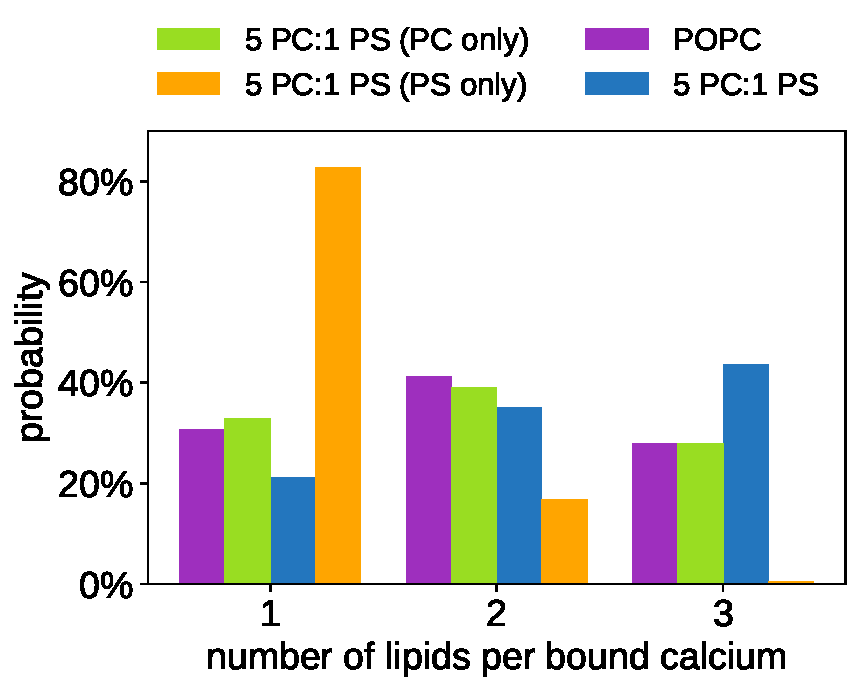
\includegraphics[width=\figwidth]{../img/stoichiometry_CaCl2_comparison_Ecc-lipids_PC-vs-PCPS.pdf} \\ 
  \caption{\label{fig:cacl_complexes} 
      Relative probabilities of existence of \ce{Ca^{2+}} complexes 
      with a certain number of lipids.  
      All lipids were taken into account with the exception of the complexes in light green and orange, 
      for which we counted only contacts with POPC resp POPS from the mixed 5\,PC:1\,PS negatively charged bilayer. 
      The calculated probabilities of the calcium-lipid complexes also reflect only POPC (light green) resp POPS (orange). 
      Probabilities were taken from simulations with comparable bulk concentrations of calcium around 250~mM. 
      Clusters of four or more lipids were not observed in either membrane. 
      Simulation data for POPC bilayers were taken directly from \cite{melcr18}. 
  } 
\end{figure} 




Relative probabilities of \ce{Ca^{2+}} complexes with a certain number of lipids are presented in Fig.~\ref{fig:cacl_complexes}. 
Calcium cations that are bound only to PC in the mixed bilayer with PS 
behave similarly as in the pure PC bilayer
maintaining comparable probabilities for clustering one, two, or even three PC lipids together. 
In contrast, PS lipids prefer 1:1 ratio with \ce{Ca^{2+}},
which may also be due to their low molar fraction in the the mixed bilayer. 
In total, however, the negatively charged membrane has its stoichiometry 
shifted towards complexes with three phospholipids and one calcium. 
This is obviously due to the presence of POPS, 
which also contributes to the pre-formed one- and two-membered clusters of POPC. 
Clusters of four or more lipids were not observed in either membrane. 

%This is also reflected in the increased probability 
%of a single phospholipid interacting with two \ce{Ca^{2+}} cations 
%compared to the neutral POPC bilayer, 
%where such a probability is almost negligable. 
% Not shown through numbers, however, I have the plots to back it. 









 
 
 





%\todo{Stationary distribution: Make a figure documenting the populations of bound \ce{Ca^{2+}} cations (like I have in the presentation) that would accompany Table \ref{tab:Ca_binding_PCPS}. 
%This will roughly correspond to the PC stoichiometry plot \ref{fig:cacl_complexes}. }




\begin{figure}[tb!]
  \centering
  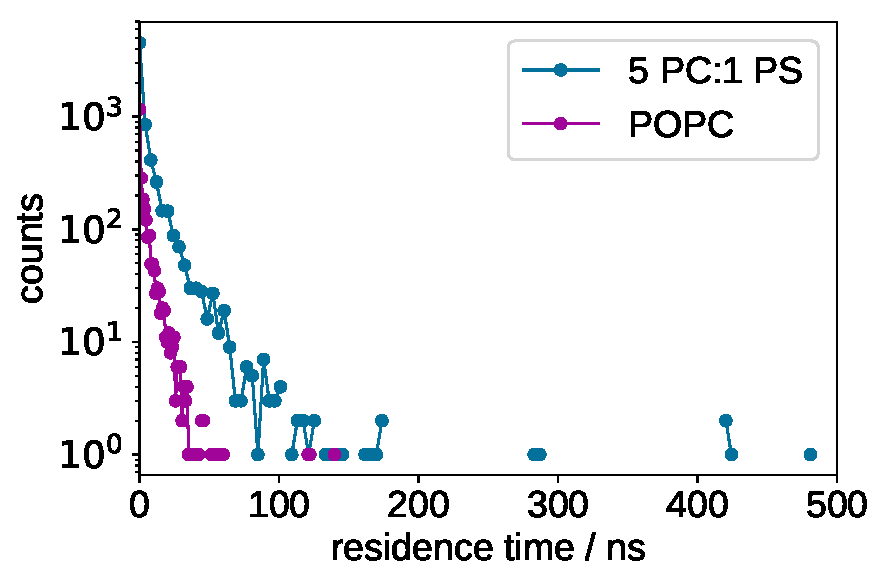
\includegraphics[width=\figwidth]{../img/histogram_bound_times_26CaCl2_comparison_PC-PCPS.pdf}
  \caption{\label{fig:hist_residence_times}
   Histograms of residence times of \ce{Ca^{2+}} 
   in a neutral membrane composed of POPC (orange)
   and in a negatively charged membrane with the composition 5\,PC:1\,PS (blue)
   from simulations with ECC-lipids and ECC-ions.
   The simulation with the neutral membrane has a bulk concentration of calcium $C_{ion} = 280\mathrm{mM}$, 
   the simulation with the negatively charged membrane has a bulk concentration of calcium $C_{ion} = 240\mathrm{mM}$. 
   In the simulation with the neutral membrane, 
   90\% of the residence times of calcium cations are
   shorter than $60\,\mathrm{ns}$, % exactly $53\,\mathrm{ns}$                                                                          
   with the longest observed residence time being $141\,\mathrm{ns}$. 
   In the simulation with the negatively charged membrane, 
   90\% of the residence times of calcium cations are
   shorter than $200\,\mathrm{ns}$, % exactly $53\,\mathrm{ns}$                                                                          
   with the longest observed residence time being $485\,\mathrm{ns}$. 
   Simulation data for POPC bilayers were taken directly from \cite{melcr18}. 
   }
\end{figure}


Timescales associated with the binding of calcium cations from solution to the membrane
are plotted for each binding event as a histogram in Fig.~\ref{fig:hist_residence_times}. 
Using these plots, we can estimate that 90\% of the residence times of any calcium cation 
will be lower than $60\,\mathrm{ns}$ for pure POPC neutral bilayer 
and shorter than $200\,\mathrm{ns}$ for the mixed 5\,PC:1\,PS negatively charged bilayer. 
The longest observed residence times in the simulations were $141\,\mathrm{ns}$ for the neutral membrane 
and $485\,\mathrm{ns}$ for the negatively charged membrane. 
Both estimates of the residence times come from simulations with comparable concentrations of around $250\mathrm{mM}$;
the simulation with the neutral membrane has a bulk concentration of calcium $C_{ion} = 280\mathrm{mM}$, 
whereas the simulation with the negatively charged membrane has a bulk concentration of calcium $C_{ion} = 240\mathrm{mM}$. 

In summary, the results from ECC-lipids suggest 
that the exchange of calcium between the POPC bilayer and the solvent 
occurs at the order of $\sim$10--100~ns, 
which is significantly faster than observed in simulations 
with other presently available non-polarizable models of lipids and ions~\citep{javanainen17, catte16}. 
Our results suggest 
that simulation trajectories with a characteristic length of several hundreds of nanoseconds 
are necessary to capture the binding of calcium to neutral POPC bilayers 
in equilibrium when more realistic \emph{polarizable} force fields are used. 
Interestingly enough, almost an order of magnitude longer simulations
are required for the negatively charged bilayers. 

 
%In addition to such estimates of the time scales, we used the Markov model on top of the simulation with the negatviely charged mixed bilayer
%to calculate the time of the mean first passage of calcium from solution to the membrane (and in reverse) resulting in $55\,\mathrm{ns}$  ($165\,\mathrm{ns}$). 

%\todo{Fluxes: committor analysis, dominant fluxes (table and figure)}
%From the spectrum of the transition matrix, we also observe that 
%the slowest transitions are associated with the binding to two or three phosphate moieties from either PC or PS,
%which are also among the states with the highest probabilities.
%The net fluxes of calcium cations from solution to such states also form a large contribution to the total flux ($\approx 45\%$). 
%\todo{Make a table and a figure of the state probabilities and fluxes to support this statement.}. 
%Analysis of the possible binding pathways of calcium cations to the negatively charged mixed bilayer 
%reveal that the cations mostly enter the membrane bound states directly from solution 
%without complicated transitions at the time scales of the order of the lag time of the Markov state model, $25\,\mathrm{ns}$. 

Provide density plots and show, where and how the cations bind to the membrane. 



 
 



 
 
 
 
 
\section{Conclusions} 

 
 
\listoftodos
 

% If you have acknowledgments, this puts in the proper section head. 
\begin{acknowledgement} 
% Put your acknowledgments here. 
P.J. acknowledges support from the Czech Science Foundation (grant no. 16-01074S)  
and from the Academy of Finland via the FiDiPro award. 
Computational resources were supplied by the Ministry of Education, Youth and Sports 
of the Czech Republic under the Projects CESNET (Project No. LM2015042) and CERIT-Scientific 
Cloud (Project No. LM2015085) provided within the program Projects of Large Research, 
Development and Innovations Infrastructures. 
O.H.S.O. acknowledges financial support from 
Integrated Structural Biology Research Infrastructure of 
Helsinki Institute of Life Science (Instruct-HiLIFE). 
\end{acknowledgement} 
 
\begin{suppinfo} 
 
%A listing of the contents of each file supplied as Supporting Information 
%should be included. For instructions on what should be included in the 
%Supporting Information as well as how to prepare this material for 
%publications, refer to the journal's Instructions for Authors. 
 
%The following files are available free of charge. 
%\begin{itemize} 
%  \item Filename: brief description 
%\end{itemize} 
 
\end{suppinfo} 
 
 
\bibliography{refs.bib} 
 
\end{document} 
 

